\documentclass[11pt]{report}
\usepackage[a4paper, width=170mm, top=25mm,bottom=25mm]{geometry}
\usepackage{fancyhdr}
\usepackage{graphics}
\usepackage{hyperref}
\usepackage{appendix}
\pagestyle{plain}
\setlength{\headheight}{12pt}
\usepackage{polyglossia}
\setmainlanguage{english}
\setotherlanguage{greek}
\usepackage{hyperref}
\usepackage{fontspec}
\renewcommand\thesection{\arabic{section}}
\setmainfont{GFS Artemisia}
\renewcommand\bibname{References}
\setcounter{secnumdepth}{5}
\usepackage{graphicx}
\usepackage{titletoc}
\usepackage{mathtools}
\usepackage{float}
\floatstyle{plaintop}
\restylefloat{table}
\usepackage{longtable}
\usepackage{array}
\usepackage{caption}
\usepackage{titlesec}
\titleformat{\chapter}[display]
  {\normalfont\bfseries}{}{-1pt}{\Huge}

\graphicspath{ {./images/} }

\title{Natural Language Processing Algorithms in Software Testing: A Systematic Literature Review}

\author{Konstantina Saketou}
\date{July 2022}
\begin{document}
  \begin{titlepage}
    \centering
    
\includegraphics[width=17cm]{images/aueb_logo.jpg}
    \vfill
    {\bfseries\Large
        ΠΤΥΧΙΑΚΗ ΕΡΓΑΣΙΑ / ΤΕΛΙΚΗ ΑΝΑΦΟΡΑ ΠΡΑΚΤΙΚΗΣ ΑΣΚΗΣΗΣ\\
        \vskip1cm
        Κωνσταντίνα Σακέτου\\
    }       
      
    
    \vfill{\bfseries\Large  
      ΕΠΙΒΛΕΠΩΝ ΚΑΘΗΓΗΤΗΣ:\\
      Παναγιώτης Λουρίδας\\ 
      \vskip1cm
      ΕΠΙΒΛΕΠΟΥΣΑ ΕΠΙΧΕΙΡΗΣΗΣ:\\
      Φωτεινή Χαρπίδη
    } 
    \vfill{\normalsize Ιούλιος 2022, Αθήνα}
    %\maketitle
  \end{titlepage}

\newpage

\begin{titlingpage}
    \clearpage 
    \vspace*{\fill} 
    \begin{center} 
        \begin{minipage}
            {\textwidth}
                \begin{center}
                    {\LARGE\bfseries Natural Language Processing in Software Testing:\\ A Systematic Literature Review\par\vspace{2\baselineskip}}
                    Konstantina Saketou\textsuperscript{1}
                    \par\vspace{\baselineskip}
                    \textsuperscript{1} Athens University of Economics and Business\par \url{www.aueb.gr}\par \end{center}
                \begin{abstract}
                    \normalsize
                        With the amount of knowledge around Natural Language Processing in Software Testing constantly growing, there is a need to provide a clear overview of the state-of-the-art 
                        technologies to the scientific community and practitioners. This Systematic Literature Review classifies recent NLP applications in Software Testing. We organize 
                        the already existing knowledge from a total of 44 scientific papers, based on Contribution Type, Software Testing Stage, 
                        Software Testing Type, Input/Output Type and NLP Techniques used in the presented context. Several findings of this review are: (1) most 
                        proposals refer to a new tool (2) many papers stick to popular NLP techniques like POS Tagging and TF-IDF to achieve their goal whereas 
                        few of them make use of more complex methods like LSTM RNNs. This review aims to make current practices and upcoming needs accessible by simplifying 
                        the searching process and providing recent organized information to be used as a starting point for further research.
                \end{abstract}
        \end{minipage} 
    \end{center} 
    \vfill 
    \clearpage

\end{titlingpage}


\startlist{toc}
\printlist{toc}{}{\chapter*{Contents}}
\newpage

\chapter*{Introduction}

Software Testing is considered a very important stage of the Software Development Lifecycle. It aims to verify and review the quality of the whole system 
under development and to make sure that it functions according to all the requirements specified by the stakeholders. There are many different types of software testing and each 
one of them has different objectives regarding the aspect of the system that will be tested. Significant aspects include the system functionality 
(Functional/Regression/Unit Testing), its overall performance (Performance/Stress Testing), its usability and also the approval from the end user and 
the degree in which he is satisfied with the system created (Acceptance Testing). Through the years, the mindset around software testing 
has developed. It is not being faced as a procedure that happens after the development stage but, on the contrary, it is now a necessary 
step towards the successful building of software. Testing happens during the whole development lifecycle, in parallel with everything else \cite{swebok}.  \\

Because of the whole growth of the software testing mindset, it has now become a process that requires many resources in order to be sucessfully
 completed and it is now one of the most expensive procedures \cite{testautomation}. For that reason, the need for integration of Automation Testing in software testing
  processes has been constantly increasing during the last years. Thanks to the use of automated test cases and automated testing in general, many benefits can be achieved, such 
  as reduction of test costs and effective reuse of code. According to a case study performed at a law-management software \cite{introautotesting}, the creation and
   use of automated GUI test cases improved significantly the whole testing process in many ways. For example, the test execution time reduced from 2 days to 1 hour and the 
   customer satisfaction increased. \\

In addition to Software Test Automation, Machine Learning methods are being also used in order to optimize automation and make the whole testing process smarter and more 
effective. More specifically, Natural Language Processing (NLP) techniques have gained significant importance with applications that focus on different stages of the software testing process. 
A plethora of approaches have been proposed, with each one of them suggesting a different method regarding, for example, the requierement analysis phase, the test case implementation or execution. 
Some of these approaches target exclusively the NLP domain whereas others incorporate it into a wider method proposal for automation testing. The kind of the proposal may also vary from a simple 
algorithm to a whole new framework. \\

This paper is a Systematic Literature Review (SLR) study about the proposed applications of NLP methods that have been published in the last two decades and refer to the Software Testing domain. 
The already existing knowledge is being organized and presented here, filtered and structured according to the different criteria identified during the scientific literature research. Through this paper, 
a current and updated context is provided, regarding the fields of NLP and Software Testing, that corresponds to recent knowledge and applications which are accessible to anyone interested in the topics discussed.
\chapter*{Background and Related Work}
This section sets the scene around the topic areas that will be discussed in this paper. Firstly, we describe basic information about the concept of NLP and we also 
provide some context related to Software Testing phases and processes. Then we briefly present studies we found that are similar to this one, compare them and consequently, 
identify the gap that this paper targets to fill. 

\section {Overview of Software Testing and NLP}

Some kind of software is now present in every form of computer that exists these days, whereas no daily activity can be completed without using one. However, this leads to the expectations we 
form for that software to be extremely high since it has to perform at its best every time it is being used. Consequently, this has created the need to ensure the overall quality and functionality of that 
software. That is the role of Software Testing. According to Bourque et al \cite{swebok}, ``\emph{Software testing consists of the dynamic verification that a program provides expected behaviors on a 
finite set of test cases, suitably selected from the usually infinite execution domain}''.\\

The testing process has four key issues \cite{swebok}. The first one is that these days it is necessary to be performed using dynamic 
inputs and not static ones in order to ensure the adaptability of the program under test. Secondly, the number of test cases created should not be infinite, although this is feasible in almost every kind 
of program and that is why it should be avoided. The third issue is that the selection of the testing techniques that will be used, should be perfomed very carefully, taking into consideration different 
aspects of the program to be tested, such as its functionality and other risks involved. Finally, the testing outcomes should be clear and easy for the test engineer to estimate if they are acceptable. 
In any other case, it means that the tests executed do not provide any substantial information for the condition and the quality of the software. \\

Another significant knowledge area that this paper focuses on is Natural Language Processing (NLP). According to Liddy E.D. \cite{liddy2001natural}, "\emph{Natural Language Processing is a theoretically motivated 
range of computational techniques for analyzing and representing naturally occurring texts at one or more levels of linguistic analysis for the purpose of achieving human-like language processing for a 
range of tasks or applications}". NLP aims to process text with a human-like approach, by transforming textual information into a structure understandable by the computer. Nowadays, NLP is an intensely growing 
field and it keeps being constantly developed. It can be applied in a variety of ways, but Information Extraction (IE) is one which we will frequently come across in this paper. \\

Information Extraction aims to identify information structures and relationships between entities included in these structures from unstructured sources \cite{infoextraction}. It is now a very well-known 
method in the NLP community with many applications in fields like machine learning, databases, web, document analysis and others. Sarawagi \cite{infoextraction} refers to these applications by separating them 
into several categories with some of them being Enterprise Applications, Personal Information Management, Scientific Applications and Web Oriented Applications. Many of the ones explained in these categories 
are related to document processing (e.g. organization of files and projects), databases (e.g. data cleaning, management of citation databases) and management of user activity on the web (e.g. comparison shopping 
websites, placement of ads in webpages etc.). The wide usage of IE is, thus, very clear based on the different types of applications refered above and it is no surprise that many of the approaches studied in 
this paper utilize IE. \\

At the below section, we present the results of the research that was made in order to map the already existing Literature Reviews related to the subject we study in this paper.

\section{Related Work}

Several other papers have been created that are close to the current research area. Four such studies where found \cite{garousi2020nlp,battina2019artificial,ahsan2017comprehensive,escalona2011overview} 
and are shortly presented in this section. Garousi et al. \cite{garousi2020nlp}, conducted a Systematic Literature Mapping regarding NLP-assisted software testing methods suggested in a pool 
of 67 papers. This mapping study classifies and overviews a list of 38 identified tools. The goal of this paper was to provide practicioners with useful information about the reasons for which 
the use of such tools might benefit their current practice. Moreover, Ahsan et al \cite{ahsan2017comprehensive}, investigated 16 papers which contained a total of 6 NLP-based techniques and 
18 tools with the same purpose. \\

Trudova et al \cite{battina2019artificial} created a Systematic Literature Review aiming to highlight the role of Artificial Intelligence in Automation Testing. 
They explore the influence of AI on the testing processes without focusing only on NLP techniques. The authors reviewed 34 papers where they identified 9 distinct software testing activities. 
The last study identified was the one conducted by Escalona et al \cite{escalona2011overview}, which focuses on NLP techniques regarding the automation of the test cases generation process. 
The analysis was performed between 24 approaches with a goal to determine the state of the art in the related area. The summary of the identified studies is displayed in Table 1. \\

\begin{table}
\resizebox{\columnwidth}{!}{%
\begin{tabular}{ |p{3cm}||p{3cm}|p{3cm}|p{3cm}|p{3cm}|p{3cm}|  }
    \hline
    \hline
    \multicolumn{6}{|c|}{Table 1. SLRs identified about NLP and Software Testing} \\
    \hline
    Title & Year & Reference & Papers studied & Focus Area & Empasis on\\
    \hline
        NLP-assisted software testing: A systematic mapping of the literature   & 2020    & \cite{garousi2020nlp}&   67 & NLP & NLP Tools \\
        \hline Artificial Intelligence in Software Test Automation: A Systematic Literature Review & 2020 & \cite{battina2019artificial} &  34 & Artificial Intelligence & Software Testing field\\
        \hline A Comprehensive Investigation of Natural Language Processing Techniques and Tools to Generate Automated Test Cases &   2017  & \cite{ahsan2017comprehensive}& 16  & NLP & Test Case Generation\\
        \hline An overview on test generation from functional requirements   & 2011 & \cite{escalona2011overview} &  24 & NLP & Test Case Generation\\
        \hline This Paper & 2022 &  & ??? & NLP & Software Testing field\\
    \hline
\end{tabular}%
}
\end{table}

% TODO: SLR in software Engineering ??

Having made a short reference to the already existing work, we notice that none of the above papers focuses on NLP techniques, different application types (tool, framework, algorithm etc.) and 
different stages of software testing at the same time. In this paper, we emphasize on studies that refer to NLP techniques, possibly propose a variety of approach types and can improve different phases 
of the Software Testing stages (e.g. requirement analysis, implementation, execution). We aim to form a broader overview of the way that NLP and Software Testing fields now cooperate to optimize 
the quality of software.
\chapter*{Research Methodology}
\addcontentsline{toc}{chapter}{Research Methodology}

\section {Research Questions}
This study aims to systematically classify the state-of-the-art in the field of Natural Language Processing combined with Software Testing 
processes. Through this procedure, this paper also targets to track possible trends and directions in current practices and techniques. In that 
way, possible future research opportunities are being also detected. To help with the categorization of the approaches and in order to give to this review a 
clear structure, we raise several research questions (RQ). These questions came up during the study of the different proposed applications. 

\subsection {RQ1: What is the proposed contribution type?}
This question refers to the kind of the approach that is being proposed. There is a big number of possible types identified. Some of them include a new tool, 
a whole framework, a simple algorithm performing a small testing-related task (or not) or it can even be a complex neural network. This paper embraces that kind of 
diversity since in that way, the different possible applications of NLP can be given prominence.

\subsection {RQ2: To what stage of Software Testing does the approach refer to?}
A significant criterion based on which we can classify the papers studied is the stage of Software Testing that they refer to. Every approach is possible to focus 
on a different testing phase. For example, some of them might refer to Requirement Analysis, Test Case Design and Development, Test Execution etc. Through this Research 
Question, we are able to observe the broader spectrum of NLP in Software Testing. Moreover, this is a great chance to take a look into other testing phases apart from 
test case creation, which seems to be the main topic of interest when it comes to NLP and Testing.

\subsection {RQ3: In which type of Software Testing is the approach being used?}
The applications studied in this paper each refer to some type of Software Testing. Some examples of these types are Manual Testing, Automation Testing and Security Testing. 
In this section, the broader contribution of NLP in Software Testing is projected, while the reader can also identify possible usages of NLP on different aspects of testing.

\subsection {RQ4: What is the input of the approach?}
There is also much interest about the different inputs of the proposed approaches. Reading through the studies, we notice a variety of data which are 
being processed to achieve the targeted result. Several applications may accept as input a UML diagram, a graph/network or text written in a Domain Specific 
Language (DSL). These are some of the different types spotted during the analysis of the papers.

\subsection {RQ5: What is the output of the approach?}
Another Research Question which is closely related with the one we just mentioned is the output type of the approaches. Since we study suggested applications 
from different stages of the Software Testing lifecycle, the outputs can vary. Depending on the stage they refer to, they can have different characteristics. 
Apart from the most common output type we will come across here, which is the test case code, some approaches may even create something which may act as 
input to another program.

\subsection {RQ6: What NLP Technique is being used?}
In that case, we are interested in the type of NLP technique that is being used to perform the proposed approach. Some applications may use the very well-known methods 
like the TF-IDF statistic and the Bag-Of-Words Model, whereas others may use something less popular or even create a completely new NLP method. By categorizing the approaches 
according to this criterion, we get a better understanding of the latest NLP method trends that are being utilized and also, we identify new needs that have emerged in the 
NLP area by studying any new proposed NLP methods.

\section {Search and Selection of papers}
The search process of the papers started by defining the corresponding search engines. The sources used were the ACM Digital Library, Scopus, 
IEEE Xplore and Google Scholar. Then, we define the search terms and keywords. The ones used were \emph{(nlp AND software testing), (nlp 
AND software testing) OR (nlp AND test automation)} and \emph{(nlp AND test automation)}. Due to the fact that the search results corresponded 
to thousands of papers, we excluded the papers that were written before the year 2000 to restrict this number. A big number of the papers that came up 
were not related at all to the current research area of interest. Also, we performed targeted search on several Conferences and Scientific Journals such 
as the International Conference on Software Engineering and the International Conference on Automated Software Engineering. The references of other previously 
published reviews were also another source utilized to track possible related studies. \\

After accessing the search results, the next step was to exclude a significant number of them and keep the ones that somehow correspond to the field we study. 
To achieve that, we read the titles and abstracts of those papers and we ended up with a total of 82 papers. Then, to further comprehend the contents of those 82 studies, 
we read and analyzed the full proposed approach of each one of them. During the reading, we excluded papers that generally refer to the field of 
Machine Learning without focusing on NLP. Also, papers that studied the broader area of Software Engineering and not specifically Testing were not 
of our interest. Many other papers studied the need for Automation in Software Testing making a short reference to the possible contribution of Machine 
Learning to that. These papers were also excluded during the searching process. \\

At that stage, all the papers of interest have been gathered and analyzed. Also, the ones that were not related to the goal of this study have been 
eliminated. After completing the above procedure, we get a final total consisting of 40 papers. 
\section {Results}

After performing a thourough analysis on the gathered scientific papers, we came up with the categorization criteria presented in chapter 3. The contribution type criterion contains the categories 
of tool, framework, algorithm and technique. Starting from the tools, these are pieces of software containing programs that are used to support an application's or a system's functionality. 
Moreover, we consider as framework a total of techniques and tools combined in order to perform and/or facilitate a task. Regarding the algorithm, it is simply a sequence of instructions given 
to the computer with the aim of solving a specific problem. Finally, in the category of the techniques and approaches, we place the papers that propose a certain way of performing a task, usually 
using already existing tools and technologies. The reviewed papers have been mapped to those types and are presented in more detail in the following sections. \\

The next criterion is the Software Testing Stage. We identified papers which refered to a varitey of phases such as Requirement Analysis, Test Planning, Implementation and also 
Reporting. As we can see, we have found applications concerning a big part of the overall Testing lifecycle. As far as the Testing Type, we have made two kinds of categorizations here. 
The first one is Manual and Automated testing, since they are both two popular test types of major significance. We next categorized the approaches based on Integration, Acceptance and Crowdsourced testing. 
However, we also encountered many papers that do not set any limilation to the applicable testing type and, thus, provide more flexibility to that part. Another criterion we indentified is the input type of 
the proposed approach. Some of the most frequent types we found is that of NL test case descriptions, use case specification documents and also test case code. We further analyze these types at the 
corresponding section. As expected, we also refer to the output type as another criterion with the most common ones being the executable code, different tyes of models or diagrams (e.g. Use case/UML diagrams) and 
others. An interesting part of this criterion that we further analyze is that several approaches generate outputs which can then be provided as input to other tools or processes in general. Last but not least, we 
have the NLP Techniques criterion where we analyze in detail the identified NLP methods used in the papers. We study that section by separating it into two categories which are techniques refering to Natural 
Language Understanding and techniques refering to Natural Language Generation. The Natural Lnaguage Understanding component also contains a small section where we present different statistical NLP measures which 
are also used in the reviewed studies.\\

In this chapter, we present the results of our Systematic Literature Review and the study of the papers identified. We separately refer to 
each criterion individually by commenting and making a short reference to the results found. In some sections and always depending on the criterion, we further analyze any 
techniques or practices encountered. 

\subsection {Contribution Type}
After reviewing all of the papers, we ended up with several contribution types proposed in their context. Our findings include tools, frameworks, algorithms and also techniques. 
In this section, we will refer to those categories that contain a big number of the papers we analyzed.\\

The first and most encountered contribution type is that of a tool. Almost 45,5\% of the studied papers suggest some sort of tool for the ease of different software testing processes. 
Some of those tools are part of the overall approach, whereas others are the main focus of the study. Some of them target the test case execution process, others focus on test case 
generation or even other areas like defects prevention and requirement analysis facilitation. Pedemonte et al \cite{pedemonte2012towards} present a way to convert manual 
functional tests into a state ready for automatic execution by using Machine Learning methods to process textual information. The tool contains semi-automatic functionality since in cases 
of textual information ambiguity, the user is prompted to interact with the tool to resolve the issue and provide the answer required to continue with the process. Another 
considerable approach is the CTRAS tool created by Hao et al \cite{8811987} which aims at the summarization of duplicate test reports in oprder to make them easily understandable 
by developers. The tool idenitfies similarities in both textual information and screenshots and comprehensibly presents them into a single report. \\

Another significant contribution type we distinguished is that of a technique or approach. As we refered earlier, this type includes any proposal of approaches, processes, techniques and any 
other alternative way of performing a certain task. We grouped them all into this category since they all somehow refer to something very similar. Specifically, 25\% of the
studied papers suggest such an approach of that type. Rajaraman et al \cite{9197868} propose in their study a way of idenitfying dependencies between tests. The authors apply Machine Learning techniques 
on log files in order to create a dependency graph which describes the connections and dependencies between the components of an application. This proposal widely facilitates the process of Integration 
Testing. We make a more detailed reference to that testing type at the corresponding section. Another paper that belongs to the technique category is that of Li et al \cite{li2022towards}. Here they propose 
an automated way for extracting knowledge from historical bug reports and for also identifying relations between them. This functionality contributes to test troubleshooting activities and it can also enhance 
the reporting stage.\\

Several other papers focused on developing a Framework to achieve their goal. Some of them refer to the topic of test case generation while others 
emphasize on the earlier stage of requirement analysis and transformation. Lafi et al \cite{9491761} created a framework which consists of different other 
processes in order to generate test cases. First of all, the use case descriptions are being processed in order to create a control flow graph and an NLP table of the 
system under test. Based on those, test paths are then generated which they will finally lead to the test case code. As far as the requirement analysis phase 
is concerned, Viggiato et al \cite{viggiato2022using} created a framework in order to help testers improve the test cases they create. This framework 
accepts test cases in natural language as input and then provides recommendations and proposed changes. More specifically, it can provide recommendations 
for the improvement of the terminology of the test cases, it can identify potentially missing test steps from those test cases and lastly, it can 
prevent test case duplicates since it is able to identify similar test cases with the one which is currently being analyzed. All of the above three 
outputs contribute immensely to the proper and effective forming of test cases by making the testers' job much easier. \\

After the analysis of the identified contribution types of the papers studied, we notice that the majority of scientific contributions revovle around 
the proposal of a tool in order to perform something new or to enhance a functionality. This is not something unexpected. Software Testing consists of many major processes, like 
test case generation, test planning, defect prevention and others, which shape all together the overall purpose of this knowledge area and are in need of improvements in order to move one step 
closer to complete automation of testing. Thus, many researchers and people interested in the field have figured out ways to enhance those methods by achieving great results.

\subsection {Software Testing Stage}
Another aspect of the papers we studied that we are interested in is the Stage of the Software Testing Lifecycle to which they apply. Some of the approaches we found refer to 
the Requirement Analysis phase, others to the Implementation and Development, Execution etc. The first one we will comment here is the Requirement Analysis. 25\% of the studies 
come up with a proposal regarding that stage and they target to enhance the processing of the test requirements and specifications. This procedure happens before the construction 
of the test cases of any form and it is a critical stage which many times determines the overall outcome of the testing cycle. Thus, it is of major importance to effectivelly 
perform the Requirement Analysis for the optimal result. \\

Sainani et al \cite{reqclass}, for example, propose a method technique which idenitfies and classifies requirements from software engineering contracts. These documents contain all 
the necessary information about the product to be developed, and therefore tested, with the desired characteristics and specifications being a part of them. The developed approach 
analyzes the contract document using different NLP techniques, which we will discuss in a further section, and outputs the different requirements of the product as well as their type. 
The output might add important information regarding the product's architecture or the importance of each feature. Based on that, developers and testers get a clear overview of what 
is worth to be tested more and also the parts that need more attention during the development and testing. This method refers to very early steps on software testing. However, 
this does not mean that such a process is not significant for a successfull testing cycle. On the contrary, it sets a concrete base for all the other stages that follow. \\

Equal importance to the Requirement Analysis stage is given by Femmer et al \cite{femmer2017rapid}. They propose a tool called Smella, which identifies Requirement Smells inside 
Requirement documents. At this point, it is worth mentioning what Requirement Smells actually are. Code smells are parts of code that need to be somehow changed in order to enhance 
its structure, complexity or comprehension \cite{fowler2018refactoring}. Consequently, Requirement Smells represent spots of Requirement Documents which need to be modified in a 
certain way in order for the product's specifications to be stated with the optimal way. For example, in a certain document it is possible to have the same requirement expressed in 
a different way. This might happen due to syntax mistakes or overall use of complex syntax in the document, which makes comprehension a harder task for the reader. This is 
the job of the Smella tool. By making good use of different NLP techniques and incorporating them into the tool, the authors managed to perform the processed described above. \\

The next stage we will refer to in this section is Software Test Planning which contains tasks like Effort Estimation and the overall planning of the roadmap of the testing 
process. Yang et al \cite{9617598} propose a method called DivClass which aims to define the optimal prioritization of test reports inspection in Crowdsource Testing. This testing type 
is covered in a next section of this chapter, so we will not further explain it here. The proposed method initially performs numerous natural language processing tasks to transform the 
test report dataset it accepts as input. Then, the similarity of those test reports is calculated and finally, based on that, the inspection priority of each one is determined. This is a 
short description of the overall method. We perform detailed reference to the different NLP techniques in Section 4.6. This approach can benefit the Software Testing process since it can 
reduce the time spent on the inspection of test reports which are not that critical or that they don't contain high importance information. On the contrary, substantial amount of time 
can be spent on inspecting test reports of higher priority. Another method which targets to make Software Testing faster is the one proposed by Tahvili et al \cite{8051381}. Their approach 
predicts the execution time of manual test cases based on their textual specifications and also on historical data from previously executed test cases. Undoubtedly this approach has a lot 
to offer to the software testing community since it enhances the manual test case execution process which most of the times it ends up requiring the most amount of time to be completed. Taking 
into account that the tester now knows the approximate execution time of the test cases, it is easier for him/her to plan the overall test cycle and create the expected timetable. \\

The testing stage which gathers the majority of the attention in the scinetific literature is the implementation/development stage. That is when the test cases are created and the whole testing 
project comes to life. At this point, it is worth mentioning that almost 63\% of the papers studied refer to that stage in some way. Because of that, we have a plethora of approach types each 
targeting a different issue. A very common task we frequently came across is the one of test case generation, usually from Requirement Documents expressed in Natural Language. Kamalakar et al 
\cite{kamalakar2013automatically}, for example, created a tool called Kirby which generates test case code from textual Requirement Specifications. Code pieces of the System Under Test 
can be also used in order for the tool to better understand the structure and semantics. However, the framework proposed by Lafi et al \cite{9491761} in order to perform the same task is different. 
This approach uses the Use Case Description of the Use Case Diagram expressed in UML. It is obvious that there is a variety of alternatives that achieve the same goals, which is the test case generation. 
Though this is not the only one we identified at the implementation stage. Viggiato et al \cite{viggiato2022using} propose a framework which aims at improving manual test case descriptions. More specifically, 
this approach accepts the test cases expressed in natural language and generates recommendations for the improvement of those descriptions. The framework recommends test case terminology improvements, 
identifies possible missing steps from those test case and it is also capable of finding potential test cases that already exist in the test code and which are similar to the one provided as input. This 
is a very powerfull approach which makes the test case implementation a piece of cake. Developing test cases based on clear, complete and comprehensive descriptions eliminates the possibility of 
mistakes and makes the whole process much faster. \\

Some of the papers we studied aim to also enhance the stage of test case execution. Pedemonte et al \cite{pedemonte2012towards} created a tool which converts manual test cases into automated ones. 
In their analysis, they emphasize on the importance of the automatic test case execution and that is why they pursuited the implementation of that task. Their approach has the ability of accepting user 
guidance if necessary, but 70\% of the test cases on which they evaluated the tool converted automatically to automated test steps without user guidance. Consequently, we see that the execution stage is also 
considered a significant one for the sucessfull completion of the Software Testing process. \\

After analyzing the testing stages on which the studied papers refer to, we should make a short reference to a less popular issue of the testing world which is that of test report manipulation. Some of the studies 
we encountered, develop approaches that aim to transform test code and outcomes into a more human-friendly format. Hao et al \cite{8811987} created a tool which not only identifies duplicate reports, but it also 
summarizes their content into a more comprehensive report. This process also happens on bug reports. On the other hand, Gonzalez et al \cite{10.1145/3283812.3283819} implemented a tool which performs a process 
opposite to what we have encountered so far in this review. The created tool converts JUnit Assertions into text written in English. Goal of this approach is to contribute to the maintenability, understandability 
and analysis of test code by reducing the existence of complex and difficult to explain code.

\subsection {Software Testing Type}
In this section of our analysis, we focus on the test type that each approach refers to. The first kind of categorization we will perform is based on the two wide groups of manual and automated tests. 
Those two testing types are widely used in software testing with each one of them serving a different purpose. Manual Testing is a well-established technique where the tester interacts with the 
application in order to validate and ensure it functions as expected and according to requirements. He performs the steps described in the test cases by manually executing them. However, this is an 
extremely expensive process and requires a big amount of resources with time and money being some of them. This gap fills the use of Automated Testing, where important stages like test generation and execution 
are performed automatically. This process significantly decreases the amount of time needed to test the product and that is the reason why Automated Testing is widely used in Agile development where 
software releases are continuous and more frequent. Moreover, a big number of papers did not set any restrictions on the testing type to which they refer and they usually include improvement recommendations for 
the overall testing process. The results of the analysis based on Testing Type are also presented in Figure 1.\\

\begin{figure}[h]
    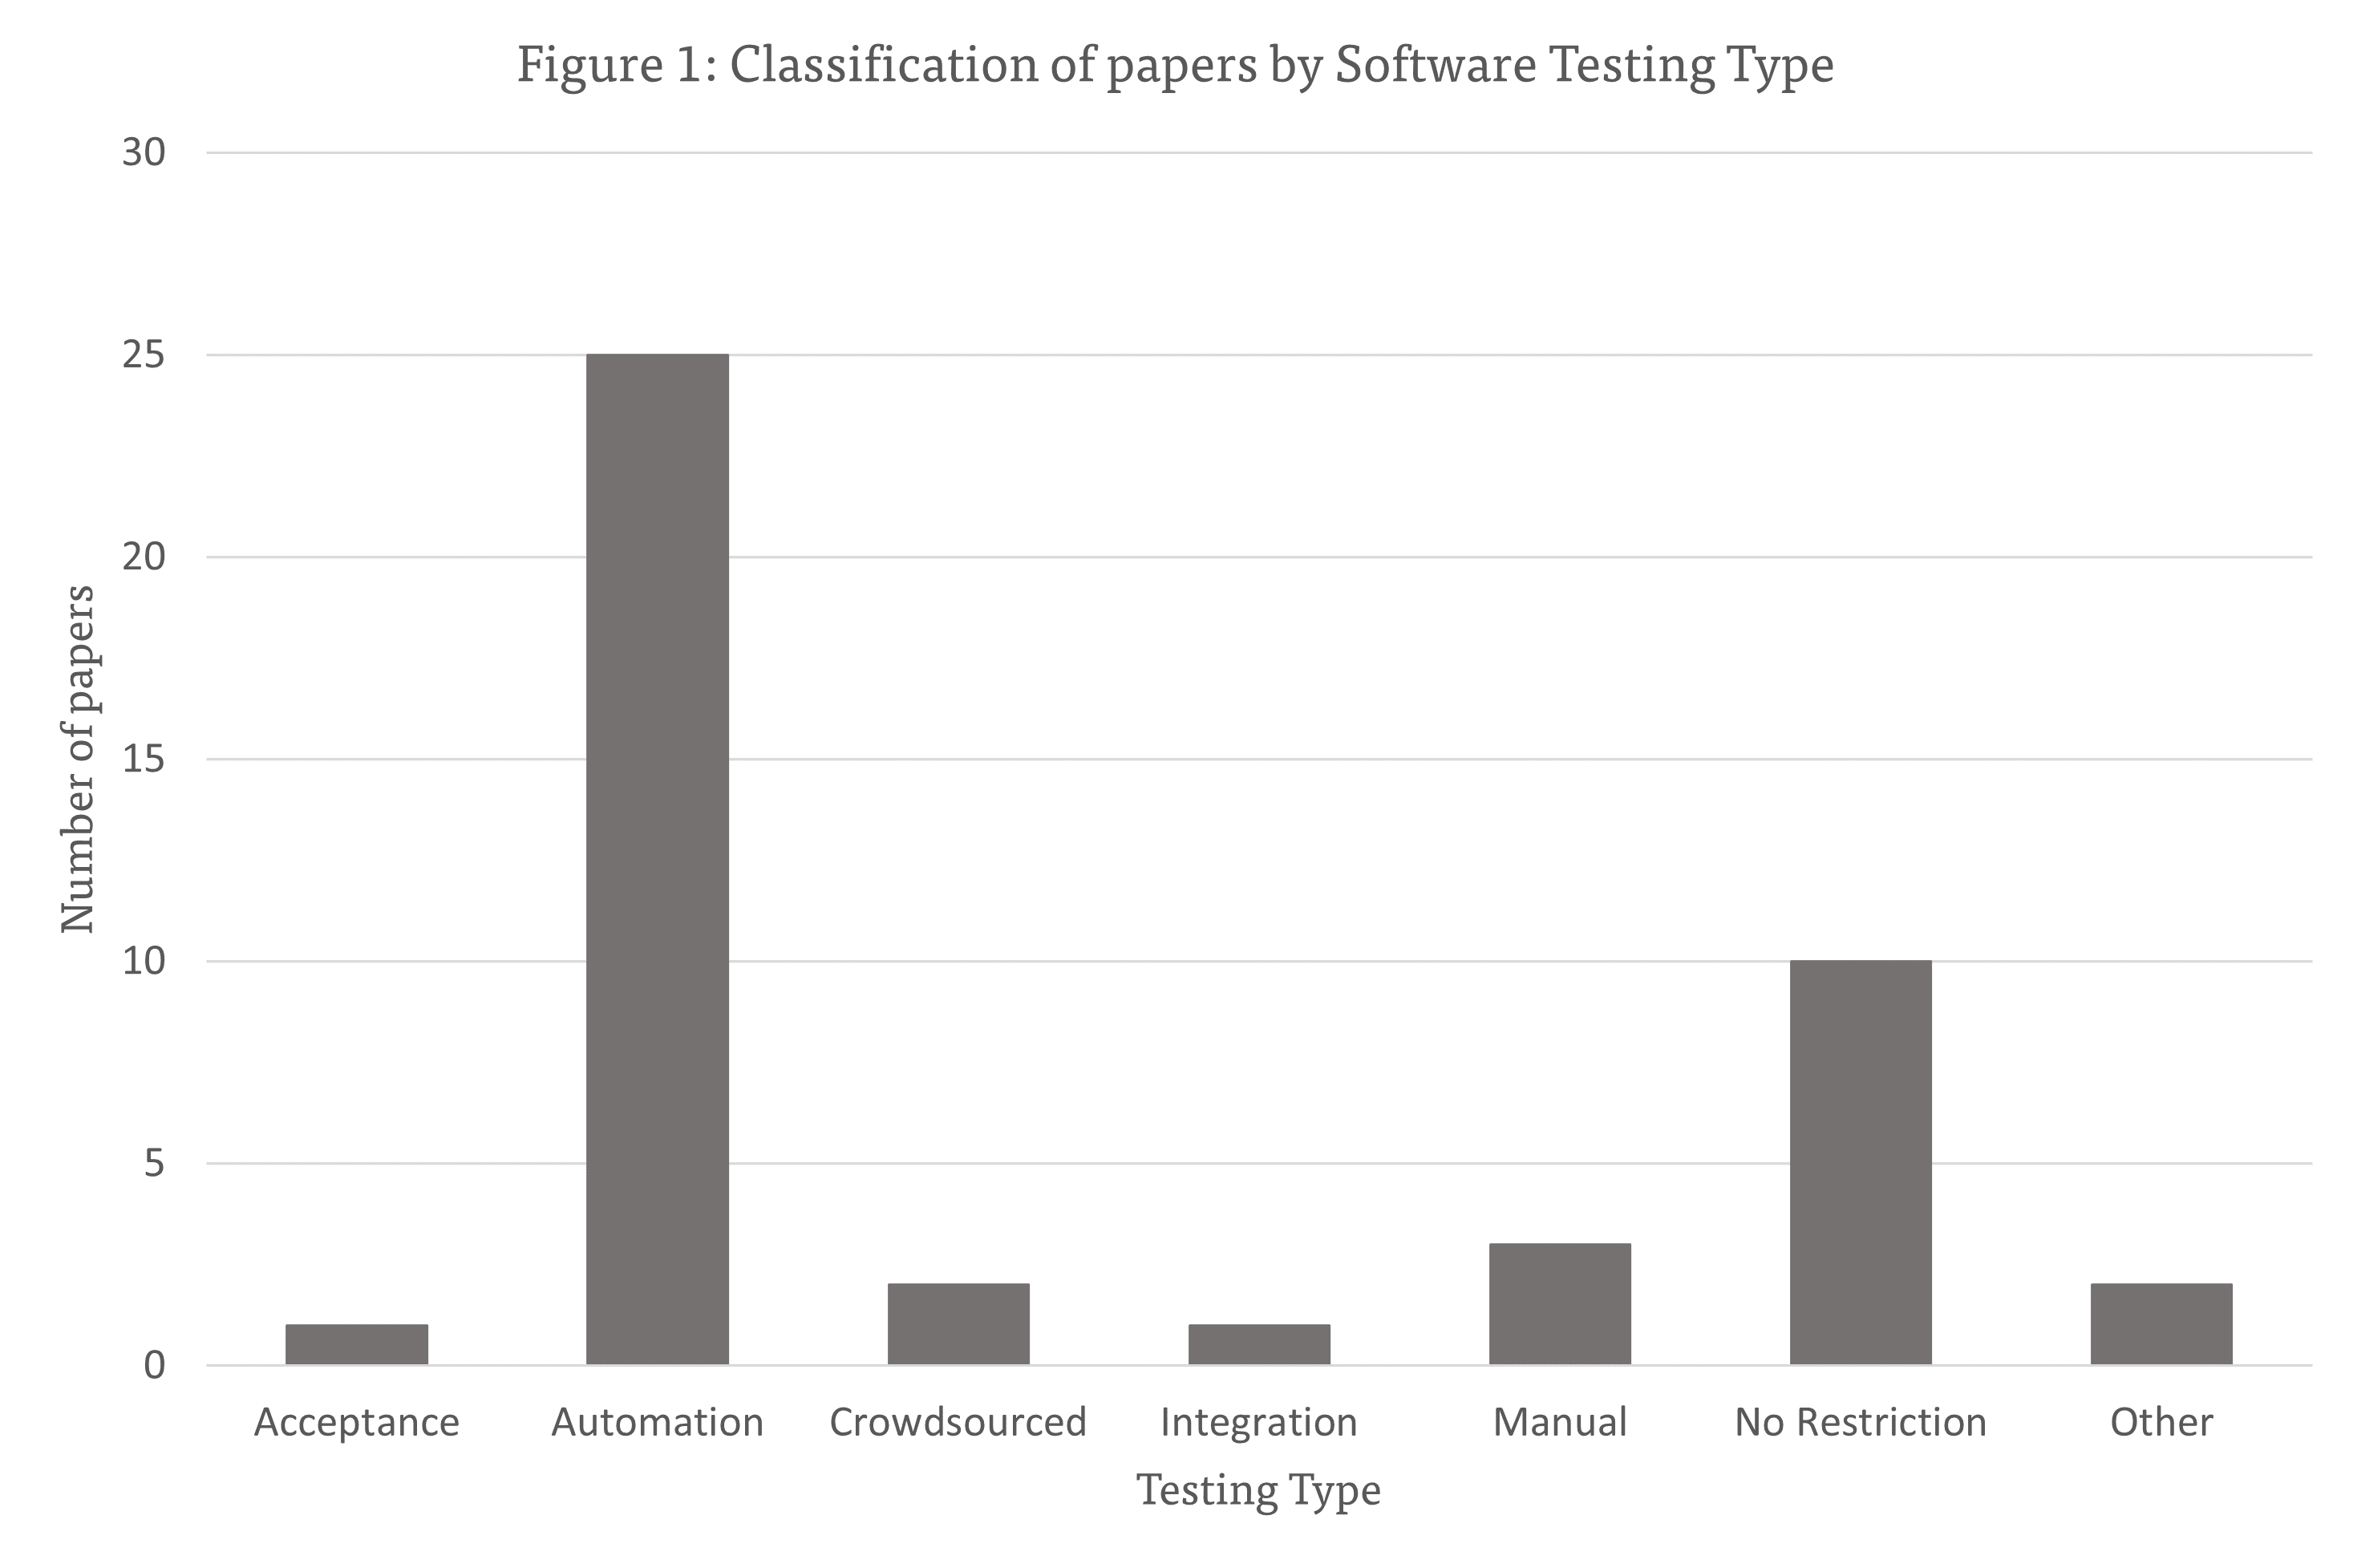
\includegraphics[width=15cm]{figure1.png}
    \centering
\end{figure}

We will firstly refer to the papers that contribute to the manual testing domain. A significant fact we notice from studying the approaches is that they refer to different phases of testing. With manual 
testing alone being a category of major importance, it is somehow reasonable for it to concern a big part of the software testing community. The Toucan4Test tool proposed by Zhang et al \cite{zhang2014systematic} facilitates 
the process of test cases forming and creation from requirements in natural language. More specifically, this approach automatically generates the test cases from specification documents in order for them to be manually 
executed from the testers. This entails that the above process outputs test cases in a comprehensive format which the executor can easily understand and that he can follow the test steps without any trouble. On 
the other hand, Tahvili et al \cite{8051381} focus on manual test planning. Since we also referred to this approach in a previous section of this chapter, here we will shortly recall the context of the proposed method. 
The authors proposed a technique which predicts the execution time of manual test cases. Such an ability is crucial for the optimized manual test execution since this is a very time consuming process. Thus, 
an effective scheduling of the test cases that are to be executed is more than important.\\

Although manual tests are a widely used testing method, automated testing has significantly grown the past few years and it continues to develop. This is also obvious from the fact that 25 out of all the papers studied 
in this review refer to this testing method. Consequently, these approaches correspond to various contribution types and testing stages. They refer to the automatic creation, forming and execution of test cases from 
different sources like requirement documents or use case diagrams. At this point, we should note that the majority of those techniques are applied during the implementation stage. One such example is the Litmus tool 
created by Dwarakanath et al \cite{litmus} which generates test cases from requirement documents without imposing any restrictions to the input language format or syntax. The tool follows a five step process. After it 
verifies that a sentence of the document is testable, the processing and generation procedure of the test case begins. A similar tool was developed by Rane et al \cite{rane2017automatic}. However, in that case the 
authors focused on optimizing the software testing process during Agile software development.\\

Apart from the above two big groups of manual and automated tests, we identified several other more specific testing types according to which we can further characterize some of the studied approaches. Those types are 
acceptance, integration and crowdsourced tests. The goal of acceptance tests is to determine whether the application meets functionality and usability criteria \cite{artoftesting}. These tests are performed by the 
end users of the application. An example of such an approach is the one proposed by Wang et al \cite{wang2020automatic} which targets the automatic generation of acceptance test cases and also, 
their automatic execution. Thus, the manual effort required is significantly reduced. Moving on to the Integration Testing type, it aims to verify that all the system modules and units communicate correctly 
to perform the functionality required \cite{leung1990study}. This testing type is performed after Unit Testing which, on the other hand, tests each module of the application separately. The technique proposed by Rajaraman et 
al \cite{9197868} targets Integration Testing. More specifically, goal of the approach is to identify interconnections and dependencies between different components of an application in order to optimize Integration Testing. 
The dependencies are determined based on the frequency of use and the importance of each component. Such characteristics exist in the application log files which are also the input of the proposed approach of 
the specific paper.\\

The third testing type we will talk about in this section is Crowdsourced Testing. Crowdsourced Testing has been growing in popularity during the last few years with many platforms having already 
been developed to serve that purpose, such as CrowdSprint\footnote{https://crowdsprint.com/crowdsourced-testing/} and TestBirds\footnote{https://www.testbirds.com/services/quality-assurance/}. 
In Crowdsourced Testing, test tasks are available online for anyone who is willing to perform them and test various software products. When the test task is completed, a test report is submitted 
describing the software's behavior \cite{cui2017should}. A paper that focuses on this testing type is one we have previously encountered written by Yang et al \cite{9617598}. The authors 
propose a method called DivClass which prioritizes the test reports coming from Crowdsource testers. Also, similar reports are identified and combined into a signle report for more effective management 
of time during test report inspection.\\

Having expanded on the Software Testing Type characteristic of this review, we notice an overall tendency of the scientific community mainly towards Automation Testing approaches and methods to further 
evolve this practice, which is currently gaining a lot of attention. We also came up to a number of papers which emphasized on a more specific testing type without making distinctions regarding the 
above categories of Automated and Manual tests. Such test types are Integration, Acceptance and Crowdsourced Testing. However, the approaches proposed there can be utilized during both automated and manual testing.

\subsection {Input Type}
The input type of the studied approaches is another significant criteria based on which we will characterize them. During our analysis, we notice 
that the nature of the input that each method accepts varies from being some sort of test case code, requirement and use case documents. However, the 
majority of the inputs represent information written in natural language.\\

We will start by referring to the approaches that need test case code in order to perform the functionality required. The tool proposed by Gonzalez et al \cite{10.1145/3283812.3283819} accepts 
as input the test code of the system under test and in particular the part of it which contains the assertions performed to check different parts of the testing 
process. After the JUnit assertions have been provided to the tool, then a summary of the code is generated. More specifically, the assertion code 
is translated into natural language statements in English. That way, the test case code obtains a comprehensive format and the maintenance 
of the test cases becomes way easier and faster. Another approach which has test case code as one of its accepted inputs is the one proposed by 
Kamalakar et al \cite{kamalakar2013automatically} which we have previously referenced again in this chapter. The goal of the approach is the generation 
of test cases from the textual descriptions of the software's functionality. However, code pieces of the software under test can be also provided as input 
to the approach in order for the tool to better understand the behavior and expected functions of the application that is being tested.\\

A very frequent input type we came across during our analysis is that of test case descriptions written in natural language. The method proposed 
by Kirinuki et al \cite{9609160} aims to facilitate the maintenance of the automated test scripts where the identification of web elements on 
web pages is necessary. In a web application elements like buttons, text input fields etc. tend to change as the application develops. That 
means that the corresponding test scripts need to constantly adapt to the new changes. However, such a process is very time consuming and 
not effective. Thus, the authors move towards script-free testing by proposing a technique where testing is performed through executable test 
cases in natural language with no need to create test scripts. Arruda et al \cite{arruda2020automation} on the other hand, developed a tool 
for test script generation which accepts as input the textual test case descriptions. This tool generates reusable code and is also able 
to adapt and integrate with different test generation frameworks for even better results.\\

The use cases and user stories of the system under test is another common input type referenced into the papers studied. That information can be provided through different forms like diagrams or 
textual documents. However, we noticed that textual descriptions outweigh the rest of the accepted input formats. The method proposed by Nogueira et al \cite{nogueira2015automatic} is one of the many which 
aim at the automatic test case generation. However, its accepted input type is the application's use cases written in a Controlled Natural Language (CNL) proposed by the authors. As stated in the paper, CNL 
is a subset of English that can be processed and translated into a formal language with possibly a different format \cite{nogueira2015automatic}. On the other hand, the approach of Mulla et al \cite{mulla2020potent} 
incorporates the user stories into software testing by specifically focusing on Agile practices. This approach exposes the importance of user story artifacts in the whole Software Testing Lifecycle by 
offering, at the same time, reusability of code, increased test case generation speed and reliability.\\

After the analysis of the different input types of the suggested approaches, we cannot question their variety and diversity. However, there is no doubt that most of them share a common characteristic. The input 
information is usually expressed in natural language in order for the corresponding method or tool to perform the task required. Since the papers we study combine Natural Language Processing Techniques with 
Software Testing, it is more than reasonable for the proposed approaches to make good use of textual information of all sorts. This is another way through which the whole contribution of the NLP knowledge area is evident.

\subsection {Output Type}
We are now moving on to the output type characteristic based on which we will continue our analysis. The different output types distinguished seem to serve multiple purposes. Several approaches generate 
results ready to be used and to enhance the testing process, whereas others create information which can then act as input into another tool, framework or process. Test reports is another frequently encountered type 
which sometimes is also seen to incorporate bug reporting information.\\

The first output type we will refer to is any form of generated code. The corresponding papers of this output type implement automatic test case generation from different input information and as a result, 
they generate executable test case code. The approach of Mueller et al \cite{inproceedings} does exactly that based on the textual requirements of the application's behavior. This is achieved by firstly 
transforming abstract textual information into a more normalized format (Textual Normal Form --- TNF) and then, the authors make good use of the UML diagram representation where the initial information 
is transferred. The UML diagram is translated into classification trees which finally, generate the output code. At this point, we should note that the generated result uses the SystemVerilog language 
to represent the corresponding outcome. According to Bergeron et al \cite{bergeron2006verification}, ``\emph{SystemVerilog is the first truly industry-standard language to cover design, assertions, 
transaction-level modeling and coverage-driven constrained random verification.}'', meaning that SystemVerilog provides a huge flexibility and support when it comes to working in areas like high-level data types, 
object oriented programming, assertions and others. That way, integration does not act as a barrier when it comes to moving and exchanging knowledge and information related to different areas each.\\

Our analysis now continues with the papers which generate information that can be then provided as input to other processes and frameworks. The method proposed by Li et al \cite{10.1145/3368089.3417067} 
identifies similar test steps by using clustering techniques. The generated output is the created clusters which contain the common test steps. Those clusters can be then taken into advantage in order 
to create or even refactor API test methods. Either by acting as input to another tool or by simply being a useful source of information to the Test Engineer, this approach achieves the development of 
simpler and clean test code.\\

Different forms of models and diagrams is another frequent output type we came across during our analysis. Some of the corresponding approaches refer to the implementation stage, but the number of methods 
that target Test and Requirement Analysis is equally noticeable. Harmain et al \cite{harmain2000cm} developed a tool called CM-Builder which aims at facilitating the process of test analysis. This tool 
accepts textual information regarding the corresponding software's requirements and then formally presents that information into a UML class diagram, consisting of the necessary object classes of the system. 
This class diagram can be then provided to any Test Analyst for further improvement. Thanks to the above process, the overall analysis of the system to be tested is being both enhanced and accelerated. 
Similar is the goal of the MaramaAIC tool developed by Kamalrudin et al \cite{kamalrudin2017maramaaic}. However, the authors focus much more on the textual requirements improvement, thus after the input 
specification documents have been provided to the tool, the generated output is either a model or diagram containing the identified recommendations. Those recommendations can be proposals to provide better consistency, 
completeness and correctness to the requirements.\\

Having concluded our analysis on the output types of the studied approaches, we see that there are two major types which stand out. Those are the executable test code and any form of model or diagram describing 
some type of information. Approaches that generate test code usually aim at the direct implementation and execution of the test cases and have taken up the mission to accelerate the overall testing process. On the 
other hand, papers that propose small and more detailed tools or methods and target the improvement of one specific stage or procedure, provide small but very useful improvements to small steps of the testing process. 
Nonetheless, both of the above directions, effectively and in their own way, enhance the testing journey. A more detailed overview about the studied papers and their matching to 
the above criteria is shown in \hyperref[table2]{Table 2} below.

\begin{longtable}{|p{3cm}|p{1cm}|p{2.5cm}|p{2.8cm}|p{2.5cm}|p{2.5cm}|}
    \caption*{Table 2. List of the studies reviewed by Contribution Type and Software Testing Stage}
    \label{table2}\\
        \hline
        Title & Ref. & Contribution Type & Software Testing Stage & Input & Output\\
        \hline
        A systematic approach to automatically derive test cases from use cases specified in restricted natural languages   & \cite{zhang2014systematic}& Tool & Requirement Analysis & NL Test Case Descriptions &
        Test Case Specifications in RTCM format \\
            \hline DASE: Document-Assisted Symbolic Execution for Improving Automated Software Testing & \cite{wong2015dase} & Tool& Requirement Analysis & Code Comments and Manual Pages & Detected bugs, Code Coverage results\\
            \hline Extracting and Classifying Requirements from Software Engineering Contracts  & \cite{reqclass} & Framework & Requirement Analysis & Software Engineering Contracts & Architectural Requirements\\
            \hline Determining Software Inter-Dependency Patterns for Integration Testing by applying Machine learning on Logs and Telemetry data
            & \cite{9197868} &  Approach/ Technique & Requirement Analysis & Log Files & Identified Dependences\\
            \hline Processing Natural Language Requirements & \cite{ambriola1997processing} & Tools& Requirement Analysis & Requirement Document & a Web-based environment aiding in NL requirements gathering  \\
            \hline Rapid Quality Assurance with Requirements Smells   & \cite{femmer2017rapid} & Tool& Requirement Analysis & Requirement Document & Identified Requirement Smells\\
            \hline CM-Builder: An Automated NL-based CASE Tool  & \cite{harmain2000cm} & Tool& Requirement Analysis & Requirement Document & UML Diagram in a semantic network\\
            \hline MaramaAIC: tool support for consistency management and validation of requirements  & \cite{kamalrudin2017maramaaic} & Tool& Requirement Analysis & Textual Requirement Specifications &
            Corrected use case model/diagram\\
            \hline Detecting System Use Cases and Validations from Documents & \cite{6693114} & Approach/ Technique& Requirement Analysis & Requirement Document & Detected use cases and rules\\
            \hline Score-Based Automatic Detection and Resolution of Syntactic Ambiguity in Natural Language Requirements & \cite{9240680} & Tool& Requirement Analysis & Requirement Documents &
            Possible word interpretations and proposal for ambiguity resolving\\
            \hline Crowdsourced Test Report Prioritization Based on Text Classification  & \cite{9617598} & Approach/ Technique& Test Planning & Test Report Dataset & Test Reports in recommended order\\
            \hline Towards Execution Time Prediction for Manual Test Cases from Test Specification  & \cite{8051381} & Approach/ Technique& Test Planning & NL Test Case Descriptions & Predicted Execution Time\\
            \hline Automatically Generating Tests from Natural Language Descriptions of Software Behavior  & \cite{kamalakar2013automatically} & Tool& Implementation & NL Test Scenario Descriptions, 
            Code pieces of developed software & Test Case Code\\
            \hline Towards Transforming User Requirements to Test Cases Using MDE and NLP & \cite{allala2019towards} & Framework& Implementation &User Requirements container (URCon) & Container with 
            annotated user requirements (AnnURCon) \\
            \hline Litmus: Generation of Test Cases from Functional Requirements in Natural Language  & \cite{litmus} & Tool& Implementation & Requirements Document & Test Case Code\\
            \hline Automation and consistency analysis of test cases written in natural language: An industrial context & \cite{arruda2020automation} & Tool& Implementation & NL Test Case Descriptions& Test Case Code\\
            \hline NAT2TESTSCR: Test case generation from natural language requirements based on SCR specifications  & \cite{carvalho2014nat2testscr} & Framework& Implementation & Requirements written in SysReq CNL& Software 
            Cost Reduction Specifications Document\\
            \hline Towards Automatic Functional Test Execution & \cite{pedemonte2012towards} & Tool& Test Execution & NL Test Case Descriptions & Adjusted Automated Test and Report\\
            \hline Abstract Flow Learning for Web Application Test Generation  & \cite{10.1145/3278186.3278194} & Tool& Implementation & NL Test Case Descriptions &ML-based trainable test flow generation system \\
            \hline A Natural Language Programming Approach for Requirements-based Security Testing & \cite{mai2018natural} & Framework& Implementation & NL Test Case Descriptions & Executable Security Test Cases\\
            \hline Automatic Generation of Acceptance Test Cases from Use Case Specifications: an NLP-based Approach & \cite{wang2020automatic} & Tool& Implementation & User Story, Test Scenario Descriptions &
             Test Case Code\\
            \hline Automatic Generation of Test Cases for Agile using Natural Language Processing & \cite{rane2017automatic} & Tool& Implementation & NL Test Case Description & Test Case Code\\
            \hline Cluster-Based Test Scheduling Strategies Using Semantic Relationships between Test Specifications & \cite{10.1145/3195538.3195540} & Framework& Implementation & Test Specifications&
            Test Case Clusters ready for scheduling\\
            \hline Clustering Test Steps in Natural Language toward Automating Test Automation & \cite{10.1145/3368089.3417067} & Framework& Implementation & NL Test Case Descriptions & Test Case Clusters\\
            \hline Generation of Executable Testbenches from Natural Language Requirement Specifications for Embedded Real-Time Systems & \cite{mueller2010generation} & Framework& Implementation & Textual 
            Requirement Specifications & SystemVerilog Code\\
            \hline Automated Test Cases Generation From Requirements Specification  & \cite{9491761} & Framework& Implementation & Use Case Description model & Test Paths, NLP table\\
            \hline Constructing Test Cases Using Natural Language Processing  & \cite{7972390} & Tool& Implementation & Functional Requirement Document & Test Case Table\\
            \hline NLP-assisted Web Element Identification Toward Script-free Testing & \cite{9609160} & Framework& Implementation & NL Test Case Descriptions & Test Procedure in NL\\
            \hline NLP-Based Requirements Formalization for Automatic Test Case Generation & \cite{inproceedings} & Approach/ Technique& Implementation & Functional Requirements&  Requirements Model\\
            \hline Syntactic Rules of Extracting Test Cases from Software Requirements  & \cite{masuda2016syntactic} & Approach/ Technique& Implementation & Functional Requirements & Syntactic Rules for Test Case Generation\\
            \hline Test Case Reuse based on ESIM Model  & \cite{chen2021test} & Approach/ Technique& Implementation & New Test Case & Test Cases Similarity\\
            \hline A Linguistic Analysis Engine for Natural Language Use Case Description and Its Application to Dependability Analysis in Industrial Use Cases
              & \cite{sinha2009linguistic} & Approach/ Technique& Implementation & Use Case Descriptions & Use Case Description Model\\
            \hline Using Natural Language Processing Techniques to Improve Manual Test Case Descriptions & \cite{viggiato2022using} & Framework& Implementation & NL Test Case Descriptions & 
            Test Case Improvement Recommendations\\
            \hline A Natural Language Processing (NLP) Framework for Embedded Systems to Automatically Extract Verification Aspects from Textual Design Requirements
            & \cite{anwar2020natural} & Framework& Implementation & Textual Design Requirements & Verification Assertions\\
            \hline Automatically Generating Precise Oracles from Structured Natural Language Specifications & \cite{8812070} & Tool& Implementation & Test Case Specifications Document & Test Case Code\\
            \hline On Learning Meaningful Assert Statements for Unit Test Cases & \cite{9283916} & Approach/ Technique& Implementation & Test and Focal method context & Assert statements\\
            \hline Building Combinatorial Test Input Model from Use Case Artefacts & \cite{preeti2017building} & Approach/ Technique& Implementation & Use Case Specifications & Test Case Model\\
            \hline Automatic generation of test cases and test purposes from natural language & \cite{nogueira2015automatic} & Tool& Implementation \& Test Execution & CNL Use Cases &Test Case Code\\
            \hline A Fine-Grained Approach for Automated Conversion of Junit Assertions to English  & \cite{10.1145/3283812.3283819} & Tool& Reporting & Test Case Code Assertions & English text  \\
            \hline CTRAS: Crowdsourced Test Report Aggregation and Summarization  & \cite{8811987} & Tool& Reporting & Test Report & Textual information and/or screenshots of duplicate tests \\
            \hline Towards the identification of bug entities and relations in bug reports & \cite{li2022towards} & Approach/ Technique& Reporting & Bug Reports & Relations between bug entities\\
            \hline Mining Historical Test Logs to Predict Bugs and Localize Faults in the Test Logs & \cite{8812113} & Tool& Test Planning & Test Logs & Identified Faults\\
            \hline The Potent Combo of Software Testing and NLP & \cite{mulla2020potent} & Algorithm& Requirement Analysis& User Stories, Test Scenario Description & Test Case Code\\
            \hline Assisted Behavior Driven Development Using Natural Language Processing & \cite{soeken2012assisted} & Tool& Implementation & Test Case Code, NL Test Case Descriptions & UML class/sequence diagram\\
        \hline
\end{longtable}

\subsection {NLP Techniques}
The field of Natural Language Processing (NLP) consists of two different components each referring to a specific task. The first one is Natural Language Understanding (NLU) and the second one is Natural Language 
Generation (NLG) \cite{liddy2001natural, khurana2017natural}. NLU involves the study and processing of text in multiple levels and aspects (e.g. syntactical, morphological etc.), in order to map the given textual 
information into useful representations. \\
NLU contains several steps which actually represent different analysis types \cite{liddy2001natural}. The first kind is Lexical Analysis which has to do with the understanding of a word's structure. 
The content of this analysis represents the Lexicon of the language which is being analyzed and contains a total of words and phrases of this language. Next we have Syntactic Analysis, during which sentences are parsed, 
based also on grammar rules, in order to analyze the relationship between words. Semantic Analysis is another NLP 
step which identifies all the possible meanings of a sentence based on the interaction of each individual meaning of the words comprising it.  For example, the sentence ``I will send a friend to my letter'' will be rejected 
during Semantic Analysis. The next type is Discourse Analysis. This kind of analysis focuses on the meaning of a text which is conveyed by the interaction of the meanings of the different sentences it contains. Lastly, we have 
Pragmatic Analysis where sentences are re-interpreted on their real meaning like, for example, the identification of the subject on sentence pronouns like ``him'', ``them'' etc.\\ As far as NLG is concerned, 
it refers to the creation of meaningful texts of different formats based on an input resource. The process consists of three phases which are identifying the goal of the task, planning on how this goal can 
be achieved taking into consideration the available resources and finally, implementing the plan created into text \cite{khurana2017natural}. The majority of the papers studied in this review perform NLU. 
However, several papers performing NLG were also identified.

\subsubsection* {Natural Language Understanding --- NLU}
We will firstly analyze the techniques used which belong to the NLU component.
Since lexical analysis aims to understand the meaning of each word individually, Part-Of-Speech (POS) tagging is one of those techniques who widely 
contribute to this process. POS tagging is used in the majority of the reviewed papers because it performs a very important task for the text processing 
procedure. Goal of this technique is to assign to each word the part of speech tag to which it belongs. POS tagging distinguishes whether a word is 
a noun, a verb, an adverb etc. In our case, it is frequently used in user requirements analysis in order to transform them into use cases which finally 
helps generate the required test cases \cite{allala2019towards, wang2020automatic, rane2017automatic, 8812070, preeti2017building, mulla2020potent}. 
Moreover, we also encountered POS tagging being used in proposed methods that focus on bug reporting and ambiguity detection in user requirements. 
Osama et al \cite{9240680}, for example, use it to assign three different types of ambiguities (semantic, syntactic and syntax) to the information identified. \\
However, several authors moved one step further from POS tagging. Specifically, we identified two papers that adopted a slightly altered approach. 
Pedemonte et al \cite{pedemonte2012towards} utilize BIO tagging \cite{ramshaw1999text}. BIO tagging facilliates the process of creating or identifying chunks of words or sentences in a text. 
In contrast to POS, BIO tagging does not assign only one label to a token, but it inserts a prefix to each token's tag which declares its position 
at a chunk. There are three possible prefixes which are B --- a tag is at the beggining of a chunk, I --- a tag is inside a chunk and O --- 
a tag does not exist in a chunk. The authors of this paper use this tagging method during the processing of functional test steps to finally transform them into 
automated tests. BIO tagging specifically helps them identify the test steps more accurately into the text, considering that each test step can 
represent a single chunk of information.\\
The second paper we found that does not use the widely known POS tagging method is the one by Carvalho et al \cite{carvalho2014nat2testscr}. The 
authors here implemented a framework for the generation of automated tests by incorporating into the process the Software Cost Reduction method, which 
detects and corrects errors during the requirement analysis phase. In this approach, a customized POS tagger was created in order for all the 
needs of the study to be satisfied. This was necessary, because the input of the approach is text written in a Controlled Natural Language (CNL) 
created by the authors called SysReq. The creation of a CNL also requires a lexicon of that language which will contain a number of its 
words and phrases. Thus, SysReq lexicon was also created. In general, it is very possible that one word has more than one meanings depending 
on its way of use inside a sentence. Since we now have a new total of textual representations, POS tagger may fail to identify and deal with 
this problem as expected. Consequently, a parser customized and adapted to SysReq-CNL was developed. This parser searches all possible 
classifications of a word into SysReq lexicon by also taking into consideration any following words that are possibly necessary in order to 
extract the suitable meaning each time. For example, if we want to analyze the phrase ``according to", the new parser will attempt to classify 
both ``according'' and also ``according to'' with the correct classification to be finally obtained from ``according to'' \cite{carvalho2014nat2testscr}.\\

We are now moving on to the Syntactic level of analysis in NLP which mainly contains parsing techniques used to identify the relationships 
between words in a text. During the parsing process, we noticed a frequent use of the Stanford CoreNLP Parser\footnote{https://stanfordnlp.github.io/CoreNLP/parser-standalone.html}. 
This is an open source software product developed by the Stanford Natural Language Processing (NLP) Group available for everyone to use. The parser generates a phrase structure tree (PST) 
from input sentences in different languages. A PST describes the relationships and dependencies between the words of a sentence as well as its 
structure. This approach is used on several papers we reviewed \cite{soeken2012assisted, rane2017automatic, 9240680}. Apart from the Stanford Parser, 
PST were also generally used in several other proposed approaches in order to achieve the same processing target as discussed above 
\cite{harmain2000cm, mulla2020potent}.\\
The Natural Language Took Kit (NLTK)\footnote{http://www.nltk.org/} is another open source project spotted being used during our analysis. 
NLTK contains many libraries and tools for performing NLP tasks --- including parsing --- using the Python programming language. The approach of 
Tahvili et al \cite{8051381} predicts the execution time of manual test cases and uses NLTK parsing to identify the activities contained in 
a manual test. Moreover, the proposal of Preeti et al \cite{preeti2017building} includes the step of parsing UML diagrams containing use 
case specifications into their analysis.\\
On the other hand, Arruda et al \cite{arruda2020automation} make use of Parsing Expression Grammar (PEG) \cite{ford2004parsing} as a 
way to deal with encountered ambiguities on the text during parsing. The authors created their own CNL syntax and rules which then incorporated 
into the PEG parser. PEG parsing is slightly different than the above parsing methods discussed since, in that case, ambiguity problems are 
solved based on the grammar rules and priority choices set during construction. Textual ambiguities also concern Sinha et al \cite{sinha2009linguistic} 
who didn't develop a new CNL to their approach. Instead, they don't restrict the textual input of their method by using shallow parsing and a 
Finite State Transducer (FST) to perform it. Shallow parsing allows us to be able to get part of the information included in the resulting parse tree. 
However, with POS tagging we can only keep the last layer of the tree which contains just the POS tags. As far as FSTs are concerned, Finite 
State methods have proven to be a very efficient and much faster way to perform different NLP tasks like lexical and syntactic analysis \cite{hobbs1997extracting}, 
especially in context-free approaches.\\

The next step in NLP is Semantic analysis, where the goal is to extract the actual or dictionary meaning of a word. For that task, we noticed 
the use of WordNet in several papers\cite{soeken2012assisted, rane2017automatic, arruda2020automation}. WordNet is a lexical database and contains semantic 
information for words in different languages available for everyone who works on NLP tasks. Sinha et al \cite{sinha2009linguistic} introduce semantic 
information to their approach through the Dictionary Concepts Annotator they created. This component uses an extensible domain dictionary to assign 
verbs to predefined actions/classes. For example, the verb ``CHANGE'' will be assigned to the following classes: ``UPDATE'' --- 78\%, ``OUTPUT'' 
--- 15\% and ``INPUT'' --- 6\% \cite{sinha2009linguistic}.\\

A worth mentioning method we identified being used in order to optimize both syntactic and semantic analysis tasks is the Word2Vec technique \cite{10.1145/3368089.3417067, reqclass, chen2021test}. 
Word2Vec \cite{mikolov2013distributed}, frequently used for word embedding processing, is a total of algorithms and architectures which transform the meaning of words into vector representations. 
That kind of representation, helps NLP tasks efficiently identify groups of similar words. The approach of Li et al \cite{10.1145/3368089.3417067} aims at clustering similar test steps in order for 
them to be assigned to the same test method and, in that way, empowering code reuse. Word2Vec significantly contributes to this paper by vectorizing the description of test sentences. The output vectors 
are then made use in word embeddings for the creation of the final test step clusters. However, Tahvili et al \cite{10.1145/3195538.3195540} use a variation of Word2Vec called Doc2Vec. 
Doc2Vec \cite{mikolov2013efficient} is ideal for vectorizing whole textual documents, in contrast to Word2Vec which vectorizes individual words. The proposed approach accepts as input test specification 
documents and clusters them in order to finally proceed to scheduling. Such a task could not be performed by Word2Vec since here we are not talking about the vectorization of small test steps but, instead, 
we vectorize a total of textual documents.\\

We will finally refer to a process identified towards the end of the NLP steps described above which is the Anaphora Resolution process. Some of the papers studied \cite{harmain2000cm, inproceedings, sinha2009linguistic} 
include this task as part of their approach. During Anaphora Resolution, pronouns are identified in the sentence and are replaced with the noun phrases they refer to. That way, the meaning of sentences becomes more clear 
and it is easier to spot dependences and semantic relationships between them. Gröpler et al \cite{inproceedings} apply Pronoun Resolution using the algorithm proposed by Lappin et al \cite{10.5555/203987.203989} in order 
to identify third person pronouns in formal requirement documents. Moreover, Sinha et al \cite{sinha2009linguistic} have dedicated a whole component of their approach to Anaphora Resolution where they use a 
specialized version of \cite{kennedy1996anaphora} to achieve the expected results.

\subsubsection* {Statistical Measures for NLP}
Apart from the different techniques used in the papers, many of them also utilize different statistical metrics to measure frequency and similarity of entities like words and sentences. 
In this section, we present the most popular metrics among the ones we identified.\\

The first measure in our analysis is TF-IDF which stands for Term Frequency - Inverse Document Frequency. TF-IDF measures the importance of a word, sentence or lemma in a document compared to its importance 
in the corresponding collection of documents or corpus \cite{infoextraction}.
Li et al \cite{10.1145/3368089.3417067} use it for this exact purpose along with Amar et al \cite{8812113}. However, apart from the classic 
TF-IDF approach, \cite{8812113} uses a variation of it called line-IDF. In this paper, the goal of the authors is to prevent bugs in code through historical test logs processing. Thus, they needed to also measure 
the importance of a log line, since in this approach, rare log lines should be strong fault indicators. Consequently, line-IDF represents the importance of a log line in a test log and is defined as:
\[ line-IDF_{l,d} = \log\frac{N}{N_l}\]
, where N is the number of logs for a test and \(N_l\) is the total number of logs that contain the line \(l\). TF-IDF is also used by Kirinuki et al \cite{9609160} during web element processing. 
More specifically, they use the metric to weigh words among elements in order to possibly identify and assign unique words to different web elements.\\

Cosine similarity is another measure we noticed being frequently used in the proposed approaches \cite{kamalakar2013automatically, 9609160, chen2021test, 8812113}. After the vectorization of the information we 
want to compare (e.g. words, phrases, lines of text), the authors use it as a way to identify any resemblance between the elements. It is defined as \cite{salton1988term}: 
\[cosine\:similarity =\cos\theta=\frac{\overrightarrow {W_1} \cdot \overrightarrow {W_2}}{|W_1||W_2|} \]
, where \(W_1\) and \(W_2\) represent the two vectorized words we are comparing.\\
The proposed approaches of \cite{chen2021test, 8812113} make use of the above measure in order to compare words in a text or document which usually contains test case descriptions.
Kamalakar et al \cite{kamalakar2013automatically} incorporate cosine similarity in their total of calculations they perform. They use a hybrid method in order to calculate similarity depending on each case 
their approach comes across, with cosine similarity being used in cases of sentence matching. Kirinuki et al \cite{9609160} use a weighted mean of two cosine similarities in order to compare a target vectorized 
string to a web element defining it like so:
\[\frac{\alpha\times cos\_sim(v_{target} + v_{text})+ cos\_sim(v_{target}+v_{attr})}{\alpha+1}\,  ,  \alpha \geq 1\]
, where \(v_{target}\) is the vectorized string and \(v_{text}\) and \(v_{attr}\) represent information of the web element's structure (e.g. class, area-hidden etc.).\\

Moving to another statistical metric, Relaxed Word-Mover's Distance (RWMD) is used in the approach of Li et al \cite{10.1145/3368089.3417067} in order to calculate the similarity of test steps. RWMD is 
a variation of Word-Mover's Distance (WMD) proposed in \cite{pmlr-v37-kusnerb15} which calculates the Euclidean distance between word embeddings. Small distance equals to dissimilarity, whereas big distance means 
that the two words are more likely to be similar. RWMD can be more efficiently computed comparing to WMD, while still providing the authors with the information requested. The authors define the RWMD distance of 
two sentences \(x\) and \(x'\) as:
\[ RWMD(x, x')=\max(\:l_1(x,x'), l_2(x,x')\:)\,   ,  where\]
\[ l_1(x, x')=\sum_{i,j=1}^{n}t_{i,j}|v_i-v_j|_2\, \:\:\:  ,    s.t.\:\:t_{i,j}=\begin{cases}
                                                                x_i, & j = argmin_j|v_i-v_j|_2\\
                                                                0,    &   otherwise \end{cases} \]
\[ l_2(x, x')=\sum_{i,j=1}^{n}t'_{i,j}|v_i-v_j|_2\, \:\:\:  ,    s.t.\:\:t'_{i,j}=\begin{cases}
                                                                x'_j, & j = argmin_j|v_i-v_j|_2\\
                                                                0,    &   otherwise \end{cases} \]
At the above formulas, we consider as \(x_i\) the normalized frequency of the word \(w_i\) in the text, whereas the vector \(v_i\) is the word embedding of \(w_i\).\\

\subsubsection* {Natural Language Generation --- NLG}
Having completed our analysis on the NLU techniques used in the studied papers, in this section we will refer to the NLG techniques identified. Specifically, we found two papers which make use of 
text generation methods and, thus, have natural language outputs. Gonzalez et al \cite{10.1145/3283812.3283819} created a code summarization tool which specifically translates JUnit assertions to English text. 
That way, the maintainability, understandability and overall analysis of software and tests is being highly improved. To achieve that, the authors used the SimpleNLG engine. SimpleNLG was introduced by Gatt et al 
\cite{gatt2009simplenlg} in order to support large-scale data-to-text NLG systems that perform summarization of numerical and symbolic data. It is a Java library which performs lexical, syntactic and 
morphological analysis on given input and it, also, provides a variety of lexical (e.g. AdverbPosition, VerbType etc.) and phrasal (e.g. Tense, InterrogationType etc.) features.\\

The second paper performing NLG is the one by Watson et al \cite{9283916} who proposed ATLAS (AuTomatic Learning of Assert Statements). ATLAS was created to predict a meaningful assert statement which can be 
used to asses the correctness of a focal method given also a test method. The ATLAS workflow consists of several steps. First of all, we have the extraction of test methods from different Java projects available 
on Github. Those methods proceed, then, to data mining tasks gathering the ones containing the ``@Test'' annotation as well as all the other declared methods of the projects. Then, during the data filtering 
stage, the methods found are separated to test and focal ones and, after the context of each focal method has been identified, ATLAS generates pairs of those test and focal methods. The relevant assert statements 
are generated as well. In order for ATLAS to learn how to successfully generate those assert statements, it uses a Recurrent Neural Network (RNN) encoder-decoder model to automate this process. RNNs are 
being frequently used in NLG tasks since it is a great way to transfer information and they can also effectively identify patterns in data.\\

In our case, the Encoder is a single layer bi-directional RNN which consists of two distinct LSTM RNNs and takes as input the tokenized test method and the context of the focal method as a stream of tokens. 
Here, the authors made use of bi-directionality in the network in order for the encoder to take into consideration both the tokens that come before and the tokens that come after as context for the token 
under analysis. This practice offers more flexibility to the overall task.\\
As far as the Decoder is concerned, it is a double layer LSTM RNN which takes as input a context vector with fixed length and transforms it into a sequence of output tokens. It uses a copy mechanism trained 
on the raw source code of the focal and test methods which facilitates the process of determining the source where the output tokens will be copied from.\\

To conclude, we see that NLG tasks can end up being pretty complex depending on the target task and the expected quality of the output. However, such tasks seem to be very popular among the NLP community 
since these days they offer a wide spectrum of possible applications in many fields and even everyday tasks. Once again, a more detailed mapping of the studied approaches is presented 
in \hyperref[table3]{Table 3} below.

\begin{longtable}{|p{4cm}|p{2.5cm}|p{4cm}|p{4cm}|}
    \caption*{ Table 3. List of the studies reviewed by NLP Techniques}
    \label{table3}\\
        \hline
        Title & Reference & NLP Techniques & NLP Tools \\
            \hline DASE: Document-Assisted Symbolic Execution for Improving Automated Software Testing & \cite{wong2015dase} &  & Stanford CoreNLP Typed dependency \\
            \hline Extracting and Classifying Requirements from Software Engineering Contracts  & \cite{reqclass} &  & Word2Vec\\
            \hline Determining Software Inter-Dependency Patterns for Integration Testing by applying Machine learning on Logs and Telemetry data
            & \cite{9197868} & Lemmatization, Tokenization, Parsing & \\
            \hline Processing Natural Language Requirements & \cite{ambriola1997processing} & Word Tagging, Fuzzy Matching & \\
            \hline Rapid Quality Assurance with Requirements Smells   & \cite{femmer2017rapid} & POS Tagging & \\
            \hline CM-Builder: An Automated NL-based CASE Tool  & \cite{harmain2000cm} & Anaphora Resolution & Stanford CoreNLP Parser\\
            \hline MaramaAIC: tool support for consistency management and validation of requirements  & \cite{kamalrudin2017maramaaic} & POS Tagging & \\
            \hline Detecting System Use Cases and Validations from Documents & \cite{6693114} & POS Tagging, Tokenization & \\
            \hline Score-Based Automatic Detection and Resolution of Syntactic Ambiguity in Natural Language Requirements & \cite{9240680} & POS Tagging & Stanford CoreNLP Parser\\
            \hline Crowdsourced Test Report Prioritization Based on Text Classification  & \cite{9617598} & Bag-of-Words Model, Synonymy Replacement & Language Technology Platform\\
            \hline Towards Execution Time Prediction for Manual Test Cases from Test Specification  & \cite{8051381} &   & Python NLTK\\
            \hline Automatically Generating Tests from Natural Language Descriptions of Software Behavior  & \cite{kamalakar2013automatically} & Cosine Similarity & \\
            \hline Towards Transforming User Requirements to Test Cases Using MDE and NLP & \cite{allala2019towards} &  POS Tagging & \\
            \hline Litmus: Generation of Test Cases from Functional Requirements in Natural Language  & \cite{litmus} &  & LinkGrammar Parser\\
            \hline Automation and consistency analysis of test cases written in natural language: An industrial context & \cite{arruda2020automation} &   & Parsing Expression Grammar (PEG), WordNet\\
            \hline NAT2TESTSCR: Test case generation from natural language requirements based on SCR specifications  & \cite{carvalho2014nat2testscr} &  Customized POS Tagger (using Software Cost Reduction method) & \\
            \hline Towards Automatic Functional Test Execution & \cite{pedemonte2012towards} & BIO Tagging & \\
            \hline Abstract Flow Learning for Web Application Test Generation  & \cite{10.1145/3278186.3278194} & LSTM RNNs & \\
            \hline A Natural Language Programming Approach for Requirements-based Security Testing & \cite{mai2018natural} & Tokenization & \\
            \hline Automatic Generation of Acceptance Test Cases from Use Case Specifications: an NLP-based Approach & \cite{wang2020automatic} &  POS Tagging & \\
            \hline Automatic Generation of Test Cases for Agile using Natural Language Processing & \cite{rane2017automatic} & POS Tagging & Stanford CoreNLP Parser, WordNet\\
            \hline Cluster-Based Test Scheduling Strategies Using Semantic Relationships between Test Specifications & \cite{10.1145/3195538.3195540} &   & Doc2Vec\\
            \hline Clustering Test Steps in Natural Language toward Automating Test Automation & \cite{10.1145/3368089.3417067} & TF-IDF, Relaxed Word-Mover's Distance & Word2Vec\\
            \hline Generation of Executable Testbenches from Natural Language Requirement Specifications for Embedded Real-Time Systems & \cite{mueller2010generation} & Lemmatization & \\
            \hline Automated Test Cases Generation From Requirements Specification  & \cite{9491761} & Control Flow Graph, NLP Table & \\
            \hline Constructing Test Cases Using Natural Language Processing  & \cite{7972390} &  Tokenization, Document Parsing & \\
            \hline NLP-assisted Web Element Identification Toward Script-free Testing & \cite{9609160} & TF-IDF, Cosine Similarity & \\
            \hline NLP-Based Requirements Formalization for Automatic Test Case Generation & \cite{inproceedings} & Anaphora Resolution & Algorithm of \cite{10.5555/203987.203989}\\
            \hline Syntactic Rules of Extracting Test Cases from Software Requirements  & \cite{masuda2016syntactic} & POS Tagging, Cosine Similarity & Penn TreeBank\\
            \hline Test Case Reuse based on ESIM Model  & \cite{chen2021test} & Cosine Similarity & Word2Vec\\
            \hline A Linguistic Analysis Engine for Natural Language Use Case Description and Its Application to Dependability Analysis in Industrial Use Cases
              & \cite{sinha2009linguistic} & Shallow Parsing, Anaphora Resolution & Finite State Transducers, Dictionary Concepts Annotator, Specialized version of \cite{kennedy1996anaphora}\\
            \hline Using Natural Language Processing Techniques to Improve Manual Test Case Descriptions & \cite{viggiato2022using} & Tokenization, n-grams, BERT-based language models & \\
            \hline A Natural Language Processing (NLP) Framework for Embedded Systems to Automatically Extract Verification Aspects from Textual Design Requirements
            & \cite{anwar2020natural} & POS Tagging, Sentence Splitting & \\
            \hline Automatically Generating Precise Oracles from Structured Natural Language Specifications & \cite{8812070} & POS Tagging & \\
            \hline On Learning Meaningful Assert Statements for Unit Test Cases & \cite{9283916} & Data Filtering, Context Understanding, LSTM RNN Decoder/Encoder model & \\
            \hline Building Combinatorial Test Input Model from Use Case Artefacts & \cite{preeti2017building} &  POS Tagging & Python NLTK\\
            \hline A systematic approach to automatically derive test cases from use cases specified in restricted natural languages   & \cite{zhang2014systematic} & NL Restriction Rules & \\
            \hline Automatic generation of test cases and test purposes from natural language & \cite{nogueira2015automatic} & Document Parsing & \\
            \hline A Fine-Grained Approach for Automated Conversion of Junit Assertions to English  & \cite{10.1145/3283812.3283819} &   & SimpleNLG\\
            \hline CTRAS: Crowdsourced Test Report Aggregation and Summarization  & \cite{8811987} & Tokenization, Synonym Identification, Jaccard Distance, PageRank & \\
            \hline Towards the identification of bug entities and relations in bug reports & \cite{li2022towards} & POS Tagging, Word Embeddings & Stanford CoreNLP\\
            \hline Mining Historical Test Logs to Predict Bugs and Localize Faults in the Test Logs & \cite{8812113} & TF-IDF, line-IDF, Cosine Similarity & \\
            \hline The Potent Combo of Software Testing and NLP & \cite{mulla2020potent} & POS Tagging & Stanford CoreNLP Parser\\
            \hline Assisted Behavior Driven Development Using Natural Language Processing & \cite{soeken2012assisted} &  & Stanford CoreNLP Parser, WordNet\\
        \hline

\end{longtable}

\section {Discussion}

This section provides an overview of the mapping that took place on the main part of this review based on the criteria discussed in Chapter 3. We discuss trends noticed 
in each criterion regarding the usage of some techniques and any frequent patterns identified at the studied proposed approaches. This, finally, leads us to several conclusions 
about the current trends of NLP applications in the Software Testing field.\\

Starting from the Contribution Type characteristic, we notice a big tendency of the scientific community in developing frameworks and tools. This probably happens because 
these type of methods align with today's needs, since many times they combine complex functionality with applications to trending business scenarios. Frameworks and tools are 
widely used by corporations and smaller businesses in order to function fast and effectively. Consequently, the scientific community adapts to today's practices and aims at 
improving and facilitating the current practice by developing methods which easily adapt to the business world.\\

Our analysis, then, proceeded to the Software Testing Stage criterion with the Implementation stage being on top of the identified types. This stage is both a very important and 
also a very time consuming part of the Testing lifecycle, and sometimes it may act as a barrier in the current Agile Development methodology followed by many organizations. A very 
big number of the papers we studied in this review have created approaches to automate the test case creation process, with that requiring very little human effort to be completed. 
That way, test case development becomes almost fully automated and the duration of the testing process decreases significantly. This again proves that the academic research keeps 
up with current trending practices in order to contribute new and useful knowledge.\\

As far as the Testing Type criterion is concerned, the vast majority of the approaches focuses on Automated Testing. As we have discussed in earlier sections of this review, the test automation 
field has been rapidly growing the last few years along with the overall tendency for automation existing in numerous parts of the corporate world and also everyday life. Taking into consideration 
the need for adaptation to new changes, the authors of many of the papers we refered here have brought automation processes one step closer to business practices. As we noticed, this is usually performed through 
the development of methods which automate tasks like test case creation and enhance different requirement analysis procedures.\\

Regarding the input type characteristic, we frequently encountered approaches that operate given documents containing natural language requirements and specifications about the tests to be developed. 
These documents act as a base for the whole testing process since they describe necessary prerequisites of the system under test. They also contain the expected functionality of the product based on which 
it is later going to be tested for. Consequently, regardless of the target of the proposed approach, requirement documents are an important source of information for software testing, which is sometimes 
difficult to make use of because of the fact that they contain natural language text that is not a very friendly data format for the computer to process. However, thanks to NLP, that kind of data types 
are being now more frequently and easily utilized.\\

Moving on to the output type, we find that test case code is one of the main data types generated by the proposed approaches. This finding aligns with the fact that many of the papers focus on the implementation 
stage, as we refered earlier. Thus, the test case generation process creates executable test code for the system under test.\\

The last criterion based on which we analyzed the papers is the NLP Techniques used in the approaches. We separated the NLP techniques in NLU and NLG methods and discussed them individually. What we eventually 
ended up on, is that the majority of the papers perform NLU tasks and use popular methods to achieve that. A widely and well-known technique used during Lexical Analysis is tagging and, more specifically, POS Tagging. 
POS Tagging identifies the part of speech to which the given words belong. However, apart from the classic use of POS Tagging, we identified several cases to which different customizations have been applied to the method. 
Those customizations are related to the choice of different tags than the classic parts of speech \cite{9240680}, whereas another paper uses BIO Tagging to further facilitate the process \cite{pedemonte2012towards}. 
Other authors even proceeded to create their own customized POS Tagger \cite{carvalho2014nat2testscr}.\\
Moreover, the use of NLP tools and libraries is also pretty often. Two distinct ones we noted are the Stanford CoreNLP library and the Python NLTK. Both of them are mainly used to support NLP parsing tasks, even though 
they provide a variety of functionalities. Word2Vec is another popular tool which turned out to be pretty popular among the papers reviewed. This tool facilitates the process of transforming the semantic representation of 
words into vectors, a task necessary in order to utilize word embeddings. To conclude, several statistical measures were also used by the authors with some of them being widely known to the NLP community. The metrics applied 
in most of the papers are TF-IDF and cosine similarity. Both of them provide an indication of the semantic similarity between two elements using their vector representations.\\
Overall, we notice a tendency to continue using long-established popular NLP methods, and customizing them if necessary to achieve the requested goal. However, this doesn't mean that attempts to incorporate more unusual 
practices have not been made. LSTM RNNs and Relaxed Word-Mover's Distance are two examples of methods which we saw being used in a low frequency among the approaches. We believe, though, that the desired complexity 
of the technique and the quality of the result play an important role in the type of method which will be used during development. During this review, we discovered that it is not necessary to use complex methods in 
order to achieve substantial results and contribute to this knowledge area. Significant approaches have been developed that highly improve testing processes by making use of simple yet effective NLP methods.

\chapter{Conclusion and Future Work}

This thesis paper classified the state-of-the-art and the practices of NLP used in the Software Testing process. We reviewed 44 scientific papers written after the year 2000 that focus on this 
knowledge area and contribute to different testing tasks. This Systematic Literature Review organizes the already existing knowledge of the scientific literature and it is a well structured source of 
information for both researchers and practitioners who operate in the software testing field.\\

Also, the incorporation of a popular Machine Learning process --- NLP --- in this knowledge area increases the level of alignment of this review with current practice and trends. By creating this study, 
we aim to make current practices and upcoming needs accessible to anyone interested. We simplified the searching process by providing recent organized information which can be used as a starting point 
for further research.\\

Given that, the present review motivates the business community to utilize outcomes and results of this paper in order to express or verify current needs and challenges faced in technical processes during 
practice. The scientific community is encouraged to use this study and the above expressed needs and challenges as a source of information in order to contribute to the solution of those problems.


\nocite{*}
\bibliographystyle{unsrt}
\bibliography{thesis/thesis_bibliography.bib}

\selectlanguage{greek}

\chapter*{Μέρος ΙΙ: Πρακτική Άσκηση}

%\tableofcontents

\chapter*{Εισαγωγή}

Η εταιρεία στην οποία διενεργήθηκε η Πρακτική μου Άσκηση είναι η Netcompany-Intasoft. Η εταιρεία ιδρύθηκε το 1996 έχοντας την επωνυμία Intrasoft International με έδρα το Λουξεμβούργο και αποτελούσε μέλος του ομίλου εταιρειών Intracom Holdings. Απο τον Οκτώβριο του 2021, ωστόσο, έγινε μέλος της Netcompany Group, η οποία αποτελεί μια από τις πιο επιτυχημένες εταιρείες πληροφορικής του Βορρά με έδρα την Δανία με έτος ίδρυσης το 2000.
\\ \\
Η Netcompany-Intrasoft προσφέρει λύσεις και υπηρεσίες πληροφορικής σε 500 οργανισμούς 70 χωρών παγκοσμίως. Οι φορείς αυτοί δραστηριοποιούνται σε διάφορους κλάδους, όπως αυτόν του Δημόσιου Τομέα, της Ευρωπαϊκής Ένωσης, Τραπεζικής και Χρηματοιοκονομικών, Κοινωνικής και Υγειονομικής Ασφάλισης, Ενέργειας, Τηλεπικοινωνιών κ.ά. Η επιχείρηση απασχολεί περίπου 2800 εργαζόμενους 50 διαφορετικών εθνικοτήτων, το οποίο επιτυγχάνει διατηρώντας γραφεία σε 13 χώρες. Έτσι, εκδηλώνεται το ενδιαφέρον της εταιρίας για διατήρηση και υιοθέτηση της πολυπολιτισμικότητας και διαφορετικότητας στο περιβάλλον της, επιτυγχάνοντας με αυτόν τον τρόπο την ανταλλαγή διαφορετικών απόψεων και τη δημιουργική συνύπαρξη των ανθρώπων της σε ένα ενιαίο πλάισιο.
\\ \\
Η εταιρεία με τοποθέτησε στο κομμάτι που παρέχει λύσεις στην Ευρωπαϊκή Επιτροπή (European Commission) και ,συγκεκριμένα, σε projects που αφορούν προϊόντα της Ευρωπαϊκής Στατιστικής Υπηρεσίας (Eurostat). Καθήκον της υπηρεσίας αυτής αποτελεί η συλλογή και δημοσίευση στατιστικών δεδομένων και μελετών που αφορούν τις χώρες της Ευρωπαϊκής Ένωσης. Οι web εφαρμογές του οργανισμού αυτού εξυπηρετούν στην διαχείριση και ανταλλαγή στατιστικών δεδομένων μεταξύ των χωρών.
\\ \\
Κατά την διάρκεια της πρακτικής άσκησης, απασχολήθηκα στο κομμάτι του Application Testing. Συγκεκριμένα, εντάχθηκα στο Software Testing Services Center - STSC, το οποίο αποτελεί ένα από τα μεγαλύτερα αυτόνομα Test Centers με πάνω από 100 Test Analysts και Test Engineers. Θέλοντας να ασχοληθώ με το κομμάτι του Test Development, απέκτησα τον ρόλο του Test Automation Engineer. Απασχολήθηκα, δηλαδή, σε οτιδήποτε αφορά testing λογισμικού μέσω αυτοματοποιημένων test scripts.
\chapter{Χαρακτηριστικά Πρακτικής Άσκησης}

\section{Software Testing Services Center}

Το Software Testing Services Center στο οποίο εντάχθηκα σκοπέυει στην διασφάλιση της ποιότητας των προϊόντων της εταιρείας αλλά και των πελατών της. Είναι υπεύθυνο για τον έλεγχο του εάν οι εφαρμογές λειτουργούν με τον αναμενόμενο και πιο αποδοτικό τρόπο και αυτό επιτυγχάνεται μέσω της εφαρμογής πολυάριθμων ειδών ελέγχων στα αντίστοιχα λογισμικά. Τα είδη των ελέγχων αυτών παραθέτονται παρακάτω:\\

\subsection*{Performance Testing}
Σκοπός του συγκεκριμένου είδους ελέγχου είναι να εξασφαλίσει την ταχύτητα, επεκτασιμότητα και σταθερότητα του λογισμικού. Συγκεκριμένα, δίνει έμφαση σε μετρικές όπως ο χρόνος απόκρισης της εφαρμογής, η αξιοπιστία, ο τρόπος με τον οποίο χρησιμοποιούνται οι πόροι αποσκοπώντας στην όσο το δυνατόν πιο αποδοτική τους αξιοποίηση. Το Performance Testing αποτελείται από τα τρία παρακάτω είδη ελέγχων.

\begin{itemize}
    \item Load Testing\\
    Στόχος του Load Testing είναι να ελέγξει το πώς ανταποκρίνεται μια εφαρμογή, ένα σύστημα σε μεγάλο αριθμό ταυτόχρονων χρηστών, οι οποίοι είναι ενεργοι και εκτελούν διάφορες ενέργειες σε αυτό.
    \item Volume Testing\\
    Όταν εφαρμόζουμε Volume Testing, παρέχουμε στην εφαρμογή μας ένα πολύ μεγάλο όγκο δεδομένων. Στόχος είναι να διαπιστωθεί έαν το σύστημα λειτουργεί όπως αναμένεται, ακόμη και με έναν μεγάλο όγκο δεδομένων. Παρά το γεγονός ότι αυτό το είδος ελέγχου μοιάζει με το Load Testing, όταν εφαρμόζουμε το δεύτερο, θέλουμε να δούμε το πώς μεταβάλλεται και επηρεάζεται η απόδοση της εφαρμογής μας όταν αυξάνεται ο όγκος δεδομένων, χωρίς να δίνουμε βάση στον τρόπο εκτέλεσης των αναμενόμενων λειτουργιών.
    \item Stress Testing\\
    Στόχος του Stress Testing είναι να εντοπίσει το ανώτατο όριο φόρτου (χρηστών, πόρων κλπ.) στο οποίο η εφαρμογή μπορεί να ανταποκριθεί αποτελεσματικά. Ακόμη, βάση δίνεται και στο πόσο ομαλή θα είναι η επαναφορά του συστήματος στο αναμενόμενο φόρτο πόρων μετά από ένα πιο απαιτητικό χρονικό διάστημα όσον αφορά την απαιτούμενη απόκριση.
\end{itemize}

\subsection*{GUI Testing}
Σε αυτό το είδος ελέγχου, στόχος είναι να διασφαλίσει ότι η γραφική διεπαφή του χρήστη είναι σχεδιασμένη σύμφωνα με τις απαιτήσεις και οδηγίες 
του πελάτη και πως μέσω αυτής εκτελούνται αποτελεσματικά όλες οι λειτουργίες της εφαρμογής. Συγκεκριμένα, ελέγχεται η εμφάνιση των οθονών, τα 
διάφορα κουμπιά, τα πεδία εισόδου δεδομένων (checkboxes, radio buttons, text input fields κλπ.), καθώς επίσης και η λειτουργικότητά τους.

\subsection*{API Testing}
Κατά το συγκεκριμένο είδος ελέγχου, διασφαλίζονται διάφορες μετρικές του συστήματός μας όπως απόδοση, λειτουργικότητα κλπ. Τα APIs δεν 
περιέχουν διεπαφή χρήστη, οπότε όλος ο έλεγχος γίνεται σε επίπεδο διαδικτυακών συναλλαγών μηνυμάτων (web transactions) μεταξύ web client και 
web server. Γενικότερα το API Testing εξυπηρετεί την μεθοδολογία Agile Software Development, καθώς προσαρμόζεται εύκολα σε νέα λειτουργικότητα, 
σε αντίθεση με τους ελέγχους μέσω γραφικής διεπαφής, οι οποίοι απαιτούν περισσότερο χρόνο για να συντηρηθούν.

\subsection*{Data Migration Testing}
Αυτός ο τύπος ελέγχου εφαρμόζεται στην περίπτωση που μια εφαρμογή ή ένα σύστημα πρόκειται να μεταφερθεί σε μια νέα υποδομή. Κατά το Migration 
Testing, διασφαλίζεται πως η εφαρμογή μεταβαίνει στη νέα υποδομή χωρίς να υπάρχει κάποια συνέπεια στην ακεραιότητα των δεδομένων. Επίσης, 
επιβεβαιώνεται πως δεν υπήρξε απώλεια δεδομένων κατά τη μεταφορά.

\subsection*{Βασικές Διαδικασίες Τμήματος}
Το Software Testing Services Center είναι υπεύθυνο για τον έλεγχο της λειτουργικότητας και απόδοσης των διαφόρων εφαρμογών που ανήκουν και χρησιμοποιούνται από τους 
Οργανισμούς και πελάτες της Netcompany-Intrasoft. Η εταιρεία μπορεί να αναλάβει να τεστάρει τόσο εφαρμογές τις οποίες αναπτύσσει εκείνη όσο και εφαρμογές που αναπτύσσονται 
από τους ίδιους τους πελάτες. Και στις δύο περιπτώσεις βασική προϋπόθεση αποτελεί αρχικά η μελέτη και ανάλυση των λειτουργικών και μη λειτουργικών απαιτήσεων του συστήματος. 
Οι λειτουργικές απαιτήσεις βοηθούν στην κατανόηση των δυνατοτήτων της εφαρμογής, ενώ οι μη λειτουργικές αποτελούν σημαντική πληροφορία για είδη ελέγχων όπως το Performance Testing 
καθώς επίσης οριοθετούν κατά ένα βαθμό την εφαρμογή σε ότι αφορά τις δυνατότητές της. Στη συνέχεια, ακολουθεί το Test Planning κατά το οποίο προγραμματίζεται η όλη διαδικασία του 
testing λαμβάνοντας υπόψη τους εκτιμώμενους χρόνους σχεδιασμού, υλοποίησης και εκτέλεσης των test cases, οι οποίοι πρέπει να συμβαδίζουν με τις αντίστοιχες προθεσμίες παράδοσης 
των ελέγχων που έχουν ζητηθεί από τον πελάτη. Συνεπώς, το Test Planning αποτελεί μια ιδιαίτερα σημαντική αλλά και κρίσιμη διαδικασία του Testing Lifecycle. Έπειτα το τμήμα προχωράει 
στον σχεδιασμό των test cases, βεβαιώνοντας ότι ικανοποιούνται όλα τα ζητούμεα κριτήρια ελέγχων που έχουν καθοριστεί από τους stakeholders. Μόλις ολοκληρωθεί ο σχεδιασμός, ακολουθεί η 
συγγραφή των automated test scripts με στόχο την υλοποίηση των test cases. Τέλος, έπεται η διαδικασία του Reporting κατά την οποία παραθέτονται τα αποτελέσματα των ελέγχων της εφαρμογής.\\

Η παραπάνω διαδικασία αποτελεί των κορμό των λειτουργιών που εκτελεί το Software Testing Services Center. Ακόμη, ακολουθείται η Agile μεθοδολογία ολοκλήρωσης των διαδικασιών με αυτό να 
συνεπάγεται συχνά παραδοτέα και ενημέρωση προς τους πελάτες. Έτσι, ο συνεχής συντονισμός και προγραμματισμός των διαδικασιών είναι κάτι απαραίτητο που συμβαίνει ανάμεσα στα μέλη του τμήματος 
μέσω αποτελεσματικής επικοινωνίας και συζήτησης.

\section*{Θέση Πρακτικής Άσκησης}
Όπως αναφέρθηκε και παραπάνω, το Software Testing Services Center αποτελείται από Test Analysts και Test Engineers. Εγώ ακολούθησα το μονοπάτι του Test Engineer, λαμβάνοντας συγκεκριμένα τον ρόλο του Test Automation Engineer, του οποίου τα καθήκοντα περιγράφονται παρακάτω.\\

\begin{itemize}
    \item Ανάλυση των σεναρίων ελέγχου, μελέτη και διερεύνηση των λειτουργικών και μη λειτουργικών απαιτήσεων του συστήματος που πρόκείται να υποβλγθούν σε έλεγχο.
    \item Ανάλυση του τι αξίζει να αυτοματοποιηθεί, μελέτη των σεναρίων ελέγχου και καθορισμός αυτών που χρίζουν αυτοματοποίησης. Τα υπόλοιπα σενάρια ελέγχου εκτελούνται manually από τους Manual Testers.
    \item Σχεδιασμός και προετοιμασία των αυτοματοποιημένων ελέγχων και δημιουργία των απαραίτητων δεδομένων ελέγχου.
    \item Οργάνωση των test cycles, εκτίμηση του απαιτούμενου χρόνου υλοποίησης και ολοκλήρωσης των καθορισμένων ελέγχων για να παραδοθεί έγκαιρα η αντίστοιχη αναφορά στους stakeholders.
    \item Προετοιμασία των στατιστικών δεδομένων από την εκτέλεση των αυτοματοποιημένων ελέγχων της εφαρμογής. Στη συνέχεια, τα δεδομένα αυτά ενσωματόνονται και υποβάλονται στους stakeholders.
\end{itemize}

\section{Μεθοδολογίες και Εργαλεία}

Η ομάδα του Software Testing Services Center χρησιμοποιεί έναν μεγάλο αριθμό εργαλείων, μεθοδολογιών και τεχνολογιών για την εκτέλεση 
των λειτουργιών του. Σε αυτό το μέρος γίνεται μια αναφορά σε όλα τα παραπάνω.

\section*{Μεθοδολογίες}
\subsection*{Behavior Driven Development}
Η Behavior Driven Development αποτελεί μια μεθοδολογία η οποία καθορίζει ουσιαστικά την συμπεριφορά του υπο ανάπτυξη συστήματος. Σύμφωνα με 
τον Smart \cite{bddbook}, η μεθοδολογία αυτή μπορεί να εφαρμοστέι τόσο σε υψηλό όσο και σε χαμηλό επίπεδο. Το υψηλό επίπεδο αναφέρεται στην περιγραφή 
των λειτουργικών απαιτήσεων του συστήματος δίνοντας έμφαση περισσότερο στο επιχειρησιακό κομμάτι. Όσον αφορά το χαμηλό επίπεδο, αυτό εστιάζει 
στην περιγραφή της συμπεριφοράς της εφαρμογής βάσει εκτελέσιμων προδιαγραφών. Ακολουθώντας αυτή την πρακτική, ο κώδικας που γράφεται είναι πιο 
εύκολα κατανοητός και συντηρίσιμος. 

\subsection*{Page Object Pattern}
Ο σχεδιασμός των test cases με τη χρήση των page objects ομαδοποιεί κατά έναν τρόπο όλα τα στοιχεία και τη λειτουργικότητα που υπάρχει σε μια 
συγκεκριμένη οθόνη μιας ιστοσελίδας και τα συγκεντρώνει σε ένα ενιαίο σημείο/κλάση. Με αυτό τον τρόπο, τυχόν αλλαγές που ίσως προκύψουν στην αντίστοιχη 
οθόνη θα απαιτούν μόνο αλλαγές στην αντίστοιχη κλάση και όχι σε πολλά σημεία του κώδικα ταυτόχρονα. Έτσι, υπάρχει ξεκάθαρος διαχωρισμός μεταξύ των στοιχείων 
που περιέχει κάθε οθόνη της εφαρμογής που ελέγχεται (πχ. κουμπιά, εικόνες κ.ά.), χωρίς να περιπλέκεται η δομή του κώδικα. Ακόμη, η λειτουργικότητα 
που προσφέρει κάθε σημείο της εφαρμογής είναι ομαδοποιημένη και πολύ πιο εύκολο να εντοπιστεί από τον αντίστοιχο tester στον κώδικα \cite{pageobject}.

\section*{Εργαλεία}
\subsection*{Java}
Η γλώσσα προγραμματισμού που χρησιμοποιείται σε αρκετά μεγάλο βαθμό για τον έλεγχο των συστημάτων και των εφαρμογών είναι η Java. Αποτελεί μια 
αντικειμενοστραφής γλώσσα, βασίζεται, δηλαδή, σε κλάσεις και αντικείμενα. Χάρη στις πολυάριθμες δυνατότητες και εφαρμογές της, δίνει την 
δυνατότητα εκτέλεσης πολλών περίπλοκων λειτουργιών και ανταποκρίνεται, έτσι, στις απαιτήσεις του τμήματος.
\subsection*{Maven}
To Maven αποτελεί ένα εργαλείο αυτοματοποίησης συνήθως διαφόρων projects γραμμένων σε Java. Εξυπηρετεί στην οργάνωση και την αποτελεσματικότερη 
διαχείριση της δομής τους. Ακόμη, διευκολύνει διάφορα στάδια του Development Life Cycle με το testing να είναι ένα από αυτά.
\subsection*{Git}
To Git αποτελεί ένα Version Control Tool, το οποίο επιτρέπει την ευκολότερη διαχείριση διαφόρων σταδίων ανάπτυξης ενός project. Εξυπηρετεί 
στον ευκολότερο εντοπισμό των αλλαγών που συμβαίνουν, διευκολύνοντας την ομαδική συνεργασία και ανάπτυξη κώδικα. Η ομάδα χρησιμοποιεί το GitLab 
για την διαχείριση των repositories.
\subsection*{Selenium}
Το εργαλείο αυτό είναι ένα από τα πιο βασικά εργαλεία που χρησιμοποιεί η ομάδα. Προσφέρει αυτοματοποίηση των φυλλομετρητών και χρησιμποιείται 
έντονα στον τομέα του Automation Testing. Μέσω των βιβλιοθηκών που παρέχει, επιτυγχάνεται η ευκολότερη και γρήγορη εκτέλεση αυτοματοποιημένων 
ελέγχων.
\subsection*{Cucumber}
Το Cucumber αποτελεί ένα εργαλείο που υποστηρίζει το Behavior Driven Development - BDD που αναφέρθηκε και παραπάνω. Χάρη στη γλώσσα Gherkin, η 
αναμενόμενη συμπεριφορά του λογισμικού εκφράζεται με πολύ απλό και κατανοητό τρόπο, ο οποίος πλησιάζει αρκετά την φυσική γλώσσα. Έτσι, γίνεται 
εύκολα κατανοητή από τον οποιονδήποτε και, συνεπώς, από τους πελάτες.
\subsection*{REST-Assured API}
Το συγκεκριμένο εργαλείο παρέχεται από την Java και εξυπηρετεί στο αυτοματοποιημένο API Testing. Συγκεκριμένα, εξυπηρετεί στον έλεγχο των REST 
Services, μέσω HTTP Requests.
\subsection*{SoapUI}
Το SoapUI αποτελεί και αυτό ένα εργαλείο για Web Service Testing. Παρ' όλα αυτά, μπορεί να χρησιμοποιηθεί και για Functional και Load Testing.
\subsection*{JMeter}
Το JMeter αποτελεί ένα εργαλείο, το οποίο χρησιμοποιείται για Performance Testing. Παρέχει, δηλαδή, στην εφαρμογή μας έναν μεγάλο όγκο 
δεδομένων με στόχο την καταγραφή του πώς αυτό ανταποκρίνεται και το πώς αποδίδει.
\chapter*{Έργα και Δραστηριότητες}
\addcontentsline{toc}{chapter}{Έργα και Δραστηριότητες}

\section*{Εισαγωγική Εκπαίδευση}
Οι δύο πρώτες εβδομάδες μετά από την έναρξη της πρακτικής μου άσκησης περιείχαν την διαδικασία εκπαίδευσής 
μου πάνω στα εργαλεία, τις μεθοδολογίες και τον τρόπο με τον οποίο εργάζεται το Software Testing Services 
Center. Η εκπαίδευση γινόταν μέσω της παρακολούθησης καταγεγραμμένων training sessions της ομάδας μου τα 
οποία  είχαν πραγματοποιηθεί στο παρελθόν και γίνονταν από τον team leader της ομάδας μου. Παράλληλα με τα 
sessions αυτά, είχα και πρακτική επαφή με το αντικείμενο πάνω στο οποίο εκπαιδευόμουν καθώς έφτιαχνα τα μικρά
 demo projects πάνω στα οποία γινόταν η εκάστοτε εκπαίδευση. Αυτά τα demo projects στη συνέχεια γινόντουσαν 
 push στο Gitlab της εταιρείας. Η δομή του «Test Engineer Learning Path» το οποίο παρακολούθησα για την 
 εκπαίδευσή μου περιείχε τα εργαλεία που χρησιμοποιεί η ομάδα, τα οποία προαναφέρθηκαν στην προηγούμενη ενότητα. \\

 Οι δυσκολίες που αντιμετώπισα κατά την διάρκεια της εκπαίδευσης αποτελούσαν κυρίως τεχνικά θέματα, όπως η πρόσβαση σε κάποιο 
 εργαλείο, και bugs τα οποία συναντούσα κατά την υλοποίηση των demo projects. Το θέμα της πρόσβασης σε κάποιο λογισμικό λυνόταν 
 σύντομα με την βοήθεια του IT Support, με τους οποίους επικοινωνούσα όταν είχα κάποιο αντίστοιχο πρόβλημα. Όσον αφορά τεχνικά θέματα 
 πάνω στα projects και τα bugs, πολλές φορές τα έλυνα εγώ, ενώ υπήρχαν περιπτώσεις στις οποίες λάμβανα βοήθεια από άλλο μέλος της ομάδας μου.

Η Εισαγωγική Εκπαίδευση διήρκησε από 21/3/2022 έως 1/4/2022.

\section*{UI Test Case Debugging - SDMXRi}
Μετά την εισαγωγική εκπαίδευση, εντάχθηκα στα projects της Eurostat ξεκινώντας με το debugging των test cases που σχετίζονταν με το User 
Interface της Web Εφαρμογής SDMX-RI. \\

«\emph{The SDMX-Reference Infrastructure (SDMX-RI) is a set of pick-and-choose building blocks and tools that allow statistical data to be 
exposed to the external world through access rights by using web services.}» 
\begin{flushright}  
    \href{https://ec.europa.eu/eurostat/cros/content/sdmx-ri_en}{- European Commission} \\
\end{flushright}

Συγκεκριμένα, η διαδικασία αποτελούνταν από την εκτέλεση ενός αυτοματοποιημένου test case, το οποίο άνοιγε την εφαρμογή στον browser και 
εκτελούσε αυτόνομα όλα τα βήματα που περιγράφονταν, ακριβώς όπως θα τα έκανε κάποιος πραγματικός χρήστης. Ωστόσο, επειδή η γραφική διεπαφή 
της εφαρμογής είχε πλέον υποστεί κάποιες αλλαγές, όπως μορφή/θέση κουμπιών, προσθήκη/αφαίρεση παραθύρων με ενημερωτικά μηνύματα κλπ, αρκετές 
από αυτές τις περιπτώσεις ελέγχου δεν εκτελούνταν επιτυχώς. Συνεπώς, μου ανατέθηκε η προσαρμογή των test cases αυτών στην νέα version της 
εφαρμογής (v 6.17.2). Οι αλλαγές που χρειάστηκε να κάνω στα test cases ήταν των παρακάτω ειδών:

\begin{itemize}
    \item Τροποποίηση των Selenium locators (XPath, CssSelector κλπ) ορισμένων elements (κουμπί, σύνδεσμος, dropdown κλπ.)
    \item Προσθήκη/αφαίρεση βημάτων (κλικ σε elements, αποδοχή/απόρριψη modals της εφαρμογής και του browser κλπ.)
    \item Προσαρμογή των δεδομένων εισόδου των test cases 
\end{itemize}

Κατά τη διάρκεια του debugging, ορισμένα test cases δεν εκτελούνταν σωστά και ο λόγος για τον οποίο συνέβαινε αυτό φαίνεται να οφειλόταν 
στην λειτουργία της εφαρμογής και όχι στα test cases. Στην περίπτωση που το πρόβλημα οφείλεται στην εφαρμογή, η ομάδα του testing οφείλει 
να ενημερώσει την development ομάδα για το bug, έτσι ώστε να το διορθώσει. Αυτό συνέβη δύο φορές κατά την διάρκεια της δραστηριότητας. 
Την πρώτη φορά, εγώ και δυο άλλα μέλη της ομάδας μου διοργανώσαμε ένα meeting για την ενημέρωση ενός από τα μέλη της development ομάδας 
για το bug. Στην δεύτερη περίπτωση, η ενημέρωση έγινε από εμένα προσωπικά στο ίδιο πάλι άτομο της development ομάδας.
Εκτός από τα παραπάνω bugs, προέκυψε και ένα πρόβλημα με το set up του Database Environment της εφαρμογής. Έτσι, διοργανώθηκε άλλο ένα 
meeting μαζί με δυο μέλη της ομάδας μου και ένα άτομο της development ομάδας, το οποίο θα μας βοηθούσε να  αντιμετωπίσουμε το πρόβλημα, όπως 
και εν τέλει έγινε.

Το παραδοτέο της παραπάνω δραστηριότητας είναι οι αλλαγές στον κώδικα που έκανα, οι οποίες αποτέλεσαν το «develop-6.17.2» branch του project 
καθώς επίσης και ο φάκελος με τα test reports από την εκτέλεση των τεστ. Η δραστηριότητα διήρκησε από τις 4/4/2022 έως τις 8/4/2022.

\section*{Δημιουργία Προσχεδίων για τα Test Cases των νέων features της εφαρμογής SDMX-Ri}
Στην συγκεκριμένη δραστηριότητα, μου ανατέθηκε να δημιουργήσω προσχέδια των test cases για την λειτουργικότητα που προστέθηκε στο SDMX-RI στην 
version 6.17. Η διαδικασία αυτή θα εξυπηρετήσει, στην συνέχεια, στο να έχει ήδη φτιαχτεί μια βάση για τα νέα test cases μόλις παραδοθούν από 
την development ομάδα στο testing για υλοποίηση. Η νέα λειτουργικότητα αναφέρεται παρακάτω:
\begin{itemize}
    \item Monitor Users (Settings): διαχείριση από τον admin της δραστηριότητας των καθορισμένων χρηστών
    \item Nsi Web Service Endpoints (Settings): διαχείριση των endpoints που αφορούν το Nsi web client
	\item Logger System (Settings): διαχείριση και προβολή των logs των http requests από/προς την εφαρμογή
	\item Browse and Download Data (Dataset menu option): περιήγηση και πρόσβαση σε στατιστικά dataset
\end{itemize}
Λόγω του ότι δεν είχαμε λάβει ακόμα πληροφορίες από την development ομάδα σχετικά με τα test cases των νέων λειτουργιών, όπως τις απαιτήσεις 
τους και τα δεδομένα εισόδου, δεν υπήρχε μεγάλο περιθώριο υλοποίησής τους. Συνεπώς, υλοποίησα κάποια πολύ αρχικά στάδια (π.χ. έλεγχος πρόσβασης 
του χρήστη στην αντίστοιχη οθόνη). Επιπλέον, η εταιρία υλοποιεί τον κώδικά της βασιζόμενη στο Page Object Model, σύμφωνα με το οποίο κάθε 
κλάση/πακέτο κλάσεων αντιπροσωπεύει μια οθόνη της εφαρμογής. Υλοποίησα, λοιπόν, και τις αντίστοιχες κλάσεις για τη νέα λειτουργικότητα σύμφωνα 
με το μοντέλο αυτό. Η δραστηριότητα διήρκησε από τις 12/4/2022 έως τις 13/4/2022.

\section*{UI Test Case Troubleshooting/Debugging – ESDEN}
Στην δραστηριότητα αυτή ασχολήθηκα με ένα άλλο project της Eurostat, το ESDEN (European Statistical Data Exchange Network), το οποίο εξυπηρετεί 
κυρίως στην διαχείριση των web endpoints και των web server/client requests για την ανταλλαγή στατιστικών δεδομένων. Συγκεκριμένα, ασχολήθηκα 
με την προσαρμογή των test cases στην τρέχουσα version της εφαρμογής, καθώς κάποιες δεν εκτελούνταν σωστά. \\

Γενικότερα, στην διαδικασία του testing και ειδικά 
σε έναν agile τρόπο ανάπτυξης, σύμφωνα με τον οποίο η ομάδα κάνει μικρότερα και συχνά deliveries του προϊόντος, η εκτέλεση των API test cases είναι κάτι που 
εφαρμόζεται πολύ περισσότερο. Οι έλεγχοι της διεπαφής χρήστη απαιτούν περισσότερο χρόνο στην συγγραφή, την εκτέλεση και την συντήρηση, ενώ ελέγχουν την ίδια 
λειτουργικότητα με τα API test cases. Συνεπώς, τα UI test cases με τα οποία ασχολήθηκα εγώ είχαν αρκετό καιρό να εκτελεστούν οπότε χρειαζόντουσαν διορθώσεις.
Ασχολήθηκα με τροποποιήσεις σε elements της διεπαφής χρήστη και με την γενικότερη ροή της λειτουργικότητας του web app. Επικοινωνούσα, επίσης, με έναν συνάδελφο 
από την ομάδα μου όποτε χρειαζόμουν βοήθεια σε κάτι ή είχα κάποια απορία, και εκείνος ήταν πάντα πρόθυμος να με βοηθήσει και να μου εξηγήσει οτιδήποτε.
Η δραστηριότητα διήρκησε από τις 13/04/2022 έως τις 20/04/2022.

\section*{Τροποποίηση ενός Test Case Scenario βάσει νέων προδιαγραφών του πελάτη - ESDEN}
Όπως αναφέρθηκε παραπάνω, το ESDEN αποτελεί μια web εφαρμογή της Eurostat μέσω της οποία επιτυγχάνεται η διαχείριση και ανταλλαγή διάφορων στατιστικών datasets. Τα dataset 
αυτά μεταφέρονται μέσω HTTP requests μεταξύ web clients και web servers, τους οποίους διασυνδέει το ESDEN. Μετά από συζήτηση με τον πελάτη, η ομάδα μου ενημερώθηκε για μια 
τροποποίηση στον τρόπο με τον οποίο η εφαρμογή διαχειρίζεται τους διάφορους web servers για να κάνει κάποιες ενέργειες. Ένα συγκεκριμένο test case ελέγχει το σενάριο αποτυχημένης 
μεταφοράς κάποιου dataset μέσω ενός μη έγκυρου web server. Οι αλλαγές που ζητήθηκαν, λοιπόν, αφορούσαν τον τρόπο με τον οποίο η εφαρμογή δημιουργεί και χρησιμοποιεί 
τον server αυτόν. \\ 

Σε συνεργασία με έναν senior test automation engineer της ομάδας μου, δουλέψαμε πάνω στην ζητούμενη τροποποίηση. Τελικά διαπιστώθηκε πως αυτό που είχε ζητηθεί 
από τον πελάτη δεν ήταν απόλυτα υλοποιήσιμο ακριβώς με τον τρόπο που ζητούνταν. Συνεπώς, ο συνεργάτης μου θα μιλούσε και πάλι με τον πελάτη για να του μεταφέρει 
την πληροφορία και ,πιθανόν, να ακολουθηθεί στο προσεχές μέλλον μια διαφορετική προσέγγιση για την αντιμετώπιση του ζητήματος. Η δραστηριότητα διήρκησε από τις 19/04/2022 έως τις 20/04/2022.

\section*{Ενημέρωηση Test Case Status Report - SDMXRi}
Στη δραστηριότητα που ακολούθησε κλήθηκα να σχηματίσω μια αναφορά, η οποία περιείχε συγκεντρωμένα όλα τα test cases τόσο για την διεπαφή χρήστη 
όσο και για το ΑΡΙ της εφαρμογής SDMXRi. Συγκεκριμένα, μου ανατέθηκε να ενημερώσω το report αυτό με την κατάσταση των test cases καθώς, επίσης, και 
με κάποιες συμπληρωματικές πληροφορίες. Δηλαδή, εκεί περιέχονταν συνολικά όλα τα test cases με το εάν έτρεχαν επιτυχώς ή όχι. Σε περίπτωση 
προβλήματος ή αποτυχίας, εφόσον το issue είχε ήδη καταχωρηθεί, υπήρχε το αντίστοιχο ticket στο Jira (εργαλείο Project Management) όπου υπήρχαν περισσότερες λεπτομέρειες για το θέμα. \\

Για την σωστή συμπλήρωση όλου του report έπρεπε να εκτελεστούν όλα τα test cases της εφαρμογής (UI \& API), τα οποία ξεπερνούσαν τα 200 σε αριθμό και να σημειωθούν τυχόν 
προβλήματα και αδυναμίες στην εκτέλεση έτσι ώστε να προωθηθούν για διόρθωση. Το report αυτό βοήθησε στη συνέχεια την ομάδα μου στον καλύτερο προγραμματισμό και οργάνωση 
των επόμενων παραδοτέων που θα γίνονταν στον πελάτη, καθώς περιείχε συγκεντρωμένη την τρέχουσα κατάσταση της δουλειάς που είχε γίνει. Η δραστηριότητα διήρκησε από τι 21/04/2022 έως τις 26/04/2022.

\section*{Δημιουργία νέων UI Test Cases - ESDEN}
Κατά την δραστηριότητα αυτή ανέλαβα να δημιουργήσω από την αρχή πέντε καινούργιες περιπτώσεις ελέγχου για την εφαρμογή ESDEN. Αυτές οι test cases 
αφορούσαν την γραφική διεπαφή της εφαρμογής. Οι προδιαγραφές των ελέγχων που έπρεπε να φτιάξω μου παραδώθηκαν μέσω του Jira στο οποίο είχαν καταχωρηθεί,  
και από όπου μπορούσα να δω ακριβώς τα βήματα που έπρεπε να εκτελετούν, τις προσυνθήκες, τις μετασυνθήκες κ.ά. όλα καθορισμένα σε φυσική γλώσσα. 
Παρακάτω αναφέρονται σύντομα τα test cases που δημιουργησα. 
\begin{itemize}
    \item Monitoring ESDEN Server\\ Η περίπτωση ελέγχου αφορά την διαχείριση του server μέσω του οποίου γίνεται η επεξεργασία και μεταφορά των αρχείων. 
    Συγκεκριμένα, εδώ ο χρήστης καλείται να μεταβάλλει το χρονικό διάστημα (file processing interval), του οποίου η εφαρμογή προβάλλει τα σταλμένα αρχεία, 
    από 1 σε 4 ώρες. Μόλις ο χρήστης αλλάξει το νούμερο αυτό, τότε η εφαρμογή αναμένεται να ανανεωθεί αυτόματα και να δείχνει πλέον τα δεδομένα αποστολών.
    \item Retry Failed Deliveries\\ Εδώ ο χρήστης καλείται να πλογηθεί στην Configuration σελίδα της εφαρμογής και να επιλέξει το αντίστοιχο κουμπί που 
    επανεκτελεί αυτόματα όλες τις ποτυχημένες αποστολές αρχείων που έχουν καταγραφεί μέχρι στιγμής.
	\item Globally Disable All Physical Routing\\ Στην περίπτωση αυτή ο χρήστης καλείται να απενεργοποιήσει αυτόματα όλα τα web server endpoints από την 
    Configuration σελίδα της εφαρμογής. Αφού ολοκληρωθεί η αντίστοιχη ενέργεια, η περίπτωση ελέγχου καλείται να επιβεβαιώσει πως όλα τα endpoints έχουν 
    πράγματι απενεργοποιηθεί επιτυχώς.
	\item Edit Physical Routing\\ Στην περίπτωση αυτή ελέγχεται η διαχείριση των endpoints. Η συγκεκριμένη test case καλεί τον χρήστη να πλοηγηθεί σε ένα
     συγκεκριμένο endpoint και να το τροποποιήσει έτσι ώστε να δέχεται μόνο requests τα οποία επιστρέφουν HTTP response status ίσο με 200, το οποίο σημαίνει 
     πως η ενέργεια έχει εκτελεστεί επιτυχώς.
    \item Add a Receive-only Global Endpoint\\ Το συγκεκριμένο test case σχετίζεται με τη διαχείριση των Global Endpoints, εκείνων δηλαδή στα οποία έχουν πρόσβαση 
    όλοι οι servers που ορίζονται στην εφαρμογή. Εδώ ο χρήστης δημιουργεί εξ ολοκλήρου ένα καινούργιο endpoint και στη συνέχεια, επιβεβαιώνεται η επιτυχής δημιουργία του.
\end{itemize}
Κατά την συγγραφή του κώδικα, συμβουλευόμουν τον supervisor και συνεργάτη μου για τυχόν διευκρινήσεις τις οποίες μου παρείχε με μεγάλη προθυμία. 
Η δημιουργία των test cases διήρκησε από τις 26/04/2022 έως τις 03/05/2022. Στη συνέχεια, ο νέος κώδικας καταχωρήθηκε στο αποθετήριο της εφαρμογής 
στο Gitlab απ' όπου και θα γινόταν η διαδικασία του Code Review. Οι ημέρες από τις 04/05/2022 έως τις 06/05/2022 περιλάμβαναν προσαρμογές και τυχόν 
διορθώσεις στις καινούργιες test cases.

\section*{Συντήρηση των UI Test Cases - SDMXRi}
Αφού είχε πλέον δημιουργηθεί το Test Case Status Report που αναφέρθηκε παραπάνω, είχαν πλέον καταγραφεί κάποια νεά προβλήματα στην λειτουργικότητα 
των test cases. Στην δραστηριότητα αυτή, ανέλαβα να κάνω μια μικρή συντήρηση στα tets cases της διεπαφής χρήστη διορθώνοντας τα προβλήματα 
που εντοπίστηκαν κατά την δημιουργία του report. Ωστόσο, κάποιες από τις διορθώσεις, αποτελούσαν ζητήματα για τα οποία ευθύνονταν η λειτουργικότητα της 
εφαρμογής. Συνεπώς, αυτό σήμαινε πως έπρεπε να υπάρξει επικοινωνία με τους developers. Έτσι, διενεργήθηκε ένα meeting μεταξύ της ομάδας μου 
και ενός developer, με τον οποίο συζητήθηκαν και επιλύθηκαν τα θέματα που εντοπίστηκαν στην λειτουργικότητα της εφαρμογής κατά την συντήρηση.
Η συντήρηση διενεργήθηκε στις 03/05/2022 και το meeting έγινε στις 06/05/2022.

\section*{API Testing Training and Troubleshooting - SDMXRi}
Στην δραστηριότητα αυτή ασχολήθηκα αποκλειστικά με το API testing. Μέχρι στιγμής δεν μου είχε δωθεί η ευκαιρία να δω με μεγάλη λεπτομέρεια 
τον τρόπο λειτουργίας των API tests. Έτσι, συνεργάστηκα με ένα από τα μέλη της ομάδας μου, το οποίο μέσω ορισμένων sessions μου έδειξε κάποια βασικά 
πράγματα για τη δομή του κώδικα, τη νοοτροπία των API tests και το πώς λειτουργούν. Μου έδειξε, επίσης, το πώς όλα τα παραπάνω χρησιμοποιούνται 
στην εφαρμογή SDMXRi. Μετά από το training, ασχολήθηκα με τη διόρθωση κάποιων bugs στα API tests που δεν έτρεχαν σωστά, σύμφωνα με το report 
που πλέον είχαμε στη διάθεσή μας. Σε συνεργασία, πάντα, με τον συνάδελφο συχνά χρειάστηκε να δουλέψουμε μαζί προσπαθώντας να βρούμε το πρόβλημα 
και το τι το προκαλεί. Η δραστηριότητα διήρκησε από τις 09/05/2022 έως τις 11/05/2022.

\section*{Διεξαγωγή εβδομαδιαίων development meetings - SDMXRi}
Στις 09/05/2022 ο Team Leader μου διοργάνωσε το πρώτο meeting που θα αφορά την πορεία όλων των projects της Eurostat. Στο meeting αυτό συμμετείχε η ομάδα 
μου που ασχολείται με τα συγκεκριμένα project καθώς επίσης και μια tester της εταιρείας από το εξωτερικό, η οποία πρόσφατα εντάχθηκε στα project της Eurostat. 
Το συγκεκριμένο meeting αποτέλεσε εν μέρει και ένα καλωσόρισμα στο νέο μέλος της ομάδας και μας έδωσε την ευκαιρία να γνωριστούμε. Η συνάντηση αυτή διεξάγεται 
εβδομαδιαία από τις 09/05 και σκοπός της είναι η οργάνωση σχετικά με την πορεία των εργασιών, η ενημέρωση των δυο team leaders για την πρόοδο 
των δραστηριοτήτων καθώς επίσης και η συζήτηση τυχόν προβληματισμών που μπορεί να προκύψουν.

\section*{Συμμετοχή σε εβδομαδιαία meetings των Eurostat Projects}
Τις πρώτες ημέρες του Ιουνίου εντάχθηκα στις συγκεκριμένες εβδομαδιαίες συναντήσεις που αφορούν όλα τα project της Eurostat με τα οποία ασχολείται η εταιρεία. Τα meetings αυτα αποτελούνται από 
τον Project Manager, τους τρεις Team Leaders που επιβλέπουν τις εφαρμογές/project της Eurostat και τρεις Test Automation Engineers. Στόχος αυτών των συναντήσεων είναι η συζήτηση για την τρέχουσα κατάσταση 
και πρόοδο των projects και η ανταλλαγή απόψεων σχετικά με την προσθήκη νέων χαρακτηριστικών και λειτουργικότητας στις εφαρμογές βάσει νέων αναγκών που επικοινωνούνται από τον πελάτη.

\section*{Test Automation Framework Refactoring - SDMXRi}
Μέχρι τις 05/05/2022 που ξεκίνησε η παρούσα δραστηριότητα, υπήρχαν δυο διαφορετικά Test Automation Frameworks για την εκδοχή της εφαρμογής που χρησιμοποιεί ο πελάτης (production version) και για εκείνη που 
αναπτύσσει η εταιρία (development version). Το γεγονός αυτό, παρότι βοήθησε στο να είναι πιο ξεκάθαρη και διαχωρισμένη η εικόνα των project, με το 
πέρασμα του χρόνου δημιουργησε την ανάγκη ένωσης των δυο αυτών frameworks σε ένα κοινό project. Αυτά τα project αποτελούν τα versions 6.10 και 6.17 του SDMXRi 
και έχουν τη δυνατότητα να χρησιμοποιηθούν με διάφορους τύπους βάσεων δεδομένων, συγκεκριμένα με MySQL, SQL Server, MariaDB και Oracle. Στο στάδιο του testing, 
συνήθως χρησιμοποιείται Oracle για την version 6.10 και MySQL για την 6.17. Το γενικότερο πλαίσιο/στόχος της δραστηριότητας είναι η διατήρηση του production 
version (6.10) σε MySQL στο master branch του αντίστοιχου repository, η προσαρμογή της version 6.10 έτσι ώστε να εκτελούνται επιτυχώς τα tests σε όλους τους διαθέσιμους τύπους βάσεων δεδομένων και 
τέλος, η δημιουργία ενός develop branch, το οποίο θα περιέχει το development version του SDMX (v6.17) εκτελέσιμο σε όλους τους διαθέσιμους τύπους βάσης δεδομένων εξίσου. \\

Στα πλαίσια, λοιπόν, της δραστηριότητας αυτής συνεργάστηκα μαζί με ένα άτομο της ομάδας μου για την ένωση των frameworks. Πρώτο βήμα αποτέλεσε η επανεκτέλεση των test 
cases με τους διάφορους πιθανούς συνδυασμούς βάσεων δεδομένων και versions, έτσι ώστε να αποκτήσουμε μια εικόνα της συνολικής κατάστασης των tests. Δημιουργήθηκε ένα 
συγκεντρωτικό spreadsheet για να μας βοηθήσει σε αυτή τη διαδικασία, το οποίο ενημερωνόταν συνεχώς με τα νέα statuses. Στη συνέχεια, ακολούθησαν κάποιες αρχικές προσαρμογές στα test cases που δεν έτρεχαν επιτυχώς. 
Οι προσαρμογές αυτές διήρκησαν κάποιες ημέρες, εφόσον πλέον μιλάμε για όλα τα test cases που έχουν γραφτεί για το SDMXRi, τα οποία ανέρχονται σε 211. Μεσολάβησαν, ακόμη, και ορισμένα meetings με άτομα από 
την development ομάδα τόσο για την αντιμετώπιση προβλημάτων σχετικά με τις βάσεις δεδομένων όσο και για την ενημέρωση από μέρους μας για νέες αδυναμίες της εφαρμογής που εντοπίστηκαν. Το αποθετήριο 
του SDMX πλέον είχε την εξής μορφή:
\begin{itemize}
    \item Master Branch\\ Το περιεχόμενο του master branch δεν άλλαξε καθόλου κατά την διαδικασία του refactoring και περιέχει μια μορφή του κώδικα που ελέγχει το SDMXRi από την οποία λείπουν, ωστόσο, ορισμένα 
    νέα χαρακτηριστικά και λειτουργικότητα. Αποτελεί τον ``κορμό'' των υπόλοιπων branches.
    \item Feature/maws-test Branch\\ Στο branch αυτό περιέχεται ο κώδικας που ελέγχει την εκδοχή του προϊόντος την οποία έχει ο πελάτης. Αυτή είναι η version 6.10 σε Oracle.
	\item Develop Branch\\ To develop branch περιέχει την νεότερη εκδοχή του SDMX (6.17) σε MySQL.
\end{itemize}
Παρά την μορφή των branches, η εναλλαγή βάσεων δεδομένων στις δυο versions είναι ιδιαίτερα εύκολη καθώς τα περιβάλλοντα εκτέλεσης του κώδικα καθορίζονται στο configuration αρχείο serenity.conf. 
Συνεπώς, αρκεί μια μικρή παρέμβαση του tester στο περιεχόμενό του για να εκτελέσει τα τεστ στον επιθυμητό συνδυασμό.\\
Η ολοκλήρωση της δραστηριότητας αυτής έδωσε μια νέα μορφή στο testing framework της εφαρμογής κάνοντάς το πιο εύκολο σε ότι αφορά την συντήρηση, ανάπτυξη και εκτέλεσή του από τον οποιοδήποτε. Είναι πλέον λιγότερο 
περίπλοκο και πιο εύκολο στην κατανόηση από κάποιον tester που δεν ξέρει σε βάθος τη δομή και λειτουργικότητα του κώδικα.\\
Η δαδικασία του refactoring ξεκίνησε στις 12/05/2022 και ολοκληρώθηκε στις 24/05/2022.

\section*{Προσαρμογή των Test Cases στους διάφορους τύπους Βάσεων Δεδομένων}
Μετά την διαδικασία του refactoring και εφόσον πλέον ο κώδικας είχε αποκτήσει μια νέα δομή, έπρεπε να ξεκινήσει η προσαρμογή των tests στους διάφορους συνδυασμούς βάσεων και στις διάφορες versions. Αυτό σημαίνει δηλαδή 
να εκτελούνται τεστ επιτυχώς ανεξάρτητα από του τι επιλογή βάσης δεδομένων έχει γίνει στην κάθε version. \\

Ωστόσο, την χρονική περίοδο που καλούνταν να ξεκινήσει η συγκεκριμένη δραστηριότητα, πλησίαζε η ημερομηνία για την οποία είχε καθοριστεί το τρίτο παραδοτέο για τον πελάτη. Στο παραδοτέο αυτό είχαν προγραμματιστεί 
να παραχωρηθούν 30 test cases συνολικά στην Eurostat. Συνεπώς, αποτελούσε προτεραιότητα να εξασφαλίσουμε ότι τα συγκεκριμένα test cases που προορίζονταν για παράδοση έτρεχαν επιτυχώς. Ελέγχοντας, λοιπόν, τα test cases 
αυτά διαπιστώσαμε πως κάποια απαιτούσαν κάποιες προσαρμογές και διορθώσεις μετά το refactoring. Προτεραιοποιήσαμε, έτσι, την διόρθωση αυτών με την οποία ασχοληθήκαμε μερικές ημέρες.\\

Μετά την προσαρμογή των test cases του παραδοτέου στον πελάτη στρέψαμε την προσοχή μας στην διόρθωση των υπόλοιπων test cases που είχαν επηρεαστεί από το refactoring. Ελάχιστες αλλαγές χρειάζονταν τα 
test της διεπαφής χρήστη, ενώ μεγαλύτερη προσοχή ήθελαν τα API tests, τα οποία ήταν και πολύ περισσότερα σε αριθμό. Κατά την δραστηριότητα αυτή, εγώ ανέλαβα την διόρθωση και εκτέλεση των test cases στο local 
environment της εταιρίας στο οποίο τρέχαμε τα test cases, ενώ ο συνάδελφός μου είχε αναλάβει την επαλήθευση της ορθότητας αυτών και την εκτέλεσή τους στο Virtual Machine που τις έτρεχε ο πελάτης. Με αυτό τον 
τρόπο, ελέγχονταν δυναμικά και άμεσα οι διορθώσεις που γίνονταν.\\

Στο σημείο αυτό, πρέπει να αναφέρουμε το είδος των διορθώσεων που χρειάστηκαν στα test cases. Ορισμένες προσαρμογές που απαιτούνταν, για παράδειγμα, περιλάμβαναν την προσθήκη if statements σε ορισμένα σημεία του 
κώδικα, τα οποία ανάλογα το είδος της βάσης δεδομένων που είχε οριστεί στο configuration file, εκτελούσαν την ίδια λειτουργία με διαφορετικό τρόπο. Για παράδειγμα, στα τεστ της διεπαφής χρήστη έπρεπε να συμπληρωθούν 
διαφορετικά πεδία, τόσο σε αριθμό όσο και σε περιεχόμενο, για την δημιουργία της σύνδεσης με την Oracle βάση συγκρητικά με εκείνη της MySQL.\\
Η δραστηριότητα αυτή ξεκίνησε στις 25/05/2022 και ολοκληρώθηκε στις 10/06/2022.

\section*{SDMX-Converter Project Troubleshooting}
Στα πλαίσια της δραστηριότητας αυτής εντάχθηκα σε ένα νέο project της Eurostat, το SDMX Converter. Η εφαρμογή αυτή επεξεργάζεται διάφορα αρχεία σε μορφή XML και XSD και τα μετατρέπει σε μορφή κατάλληλη για χρήση από 
άλλες εφαρμογές του Οργανισμού μέσω HTTP Requests. Συνεπώς, ασχολήθηκα με το API της εφαρμογής. Μου ανατέθηκε να ασχοληθώ με ένα συγκεκριμένο πρόβλημα που υπήρχε, σύμφωνα με το οποίο η εφαρμογή δεν μπορούσε να 
συνδεθεί σε ορισμένες διευθύνσεις και να αποκτήσει πρόσβαση σε κάποια αρχεία που όριζε το test case. Κατά την δραστηριότητα αυτή απασχολήθηκα με το αντικείμενο του networking, της client-server επικοινωνίας και 
ανταλλαγής δεδομένων μέσω REST APIs. Η δραστηριότητα ξεκίνησε στις 11/06/2022 και ολοκληρώθηκε στις 20/06/2022.
\chapter*{Χρονικός Προγραμματισμός του Έργου}
\addcontentsline{toc}{chapter}{Χρονικός Προγραμματισμός του Έργου}

Στο κεφάλαιο αυτό παρουσιάζεται ο συνολικός χρονικός προγραμματισμός των δραστηριοτήτων της πρακτικής άσκησης. Οι δραστηριότητες φαίνονται στον παρακάτω πίνακα, καθώς επίσης 
και στο Gantt Chart στο τέλος της σελίδας.\\

\section{Χρονικός Προγραμματισμός Δραστηριοτήτων}
\begin{figure}[h]
    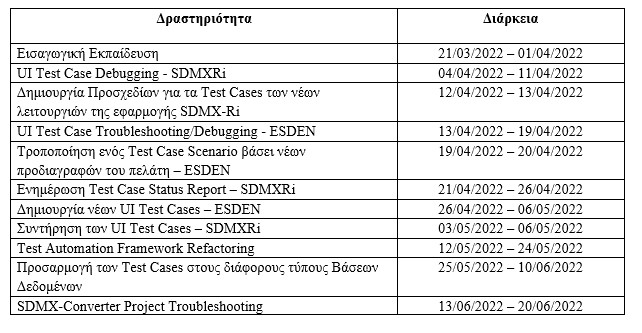
\includegraphics[width=15cm]{internship_activities_table.jpg}
    \centering
\end{figure}

\section{Gantt Chart}
\begin{figure}[h]
    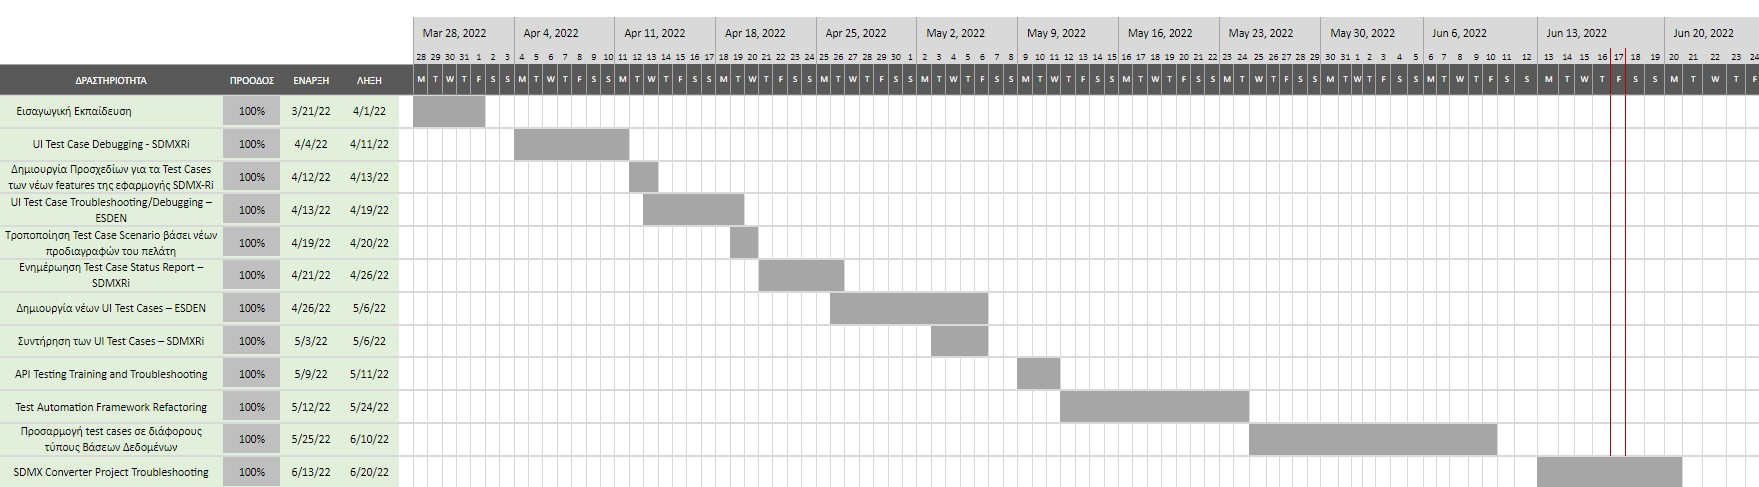
\includegraphics[width=17cm]{internship_gantt_chart.jpg}
    \centering
\end{figure}

\end{document}
